% ! TEX root = ./mechanics.tex

\chapter{超静定次数}
\section{基本原则}
\begin{enumerate}
\item 平面内的任意一个刚性杆件,如果要静定就要三个约束。如果没有约束就看成$\displaystyle -3$次静定。
\begin{figure}[!ht]
	\centering
\tikzset{every picture/.style={line width=0.75pt}} %set default line width to 0.75pt        

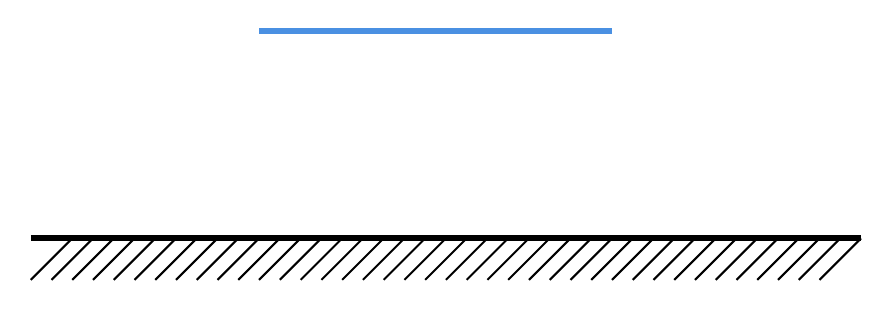
\begin{tikzpicture}[x=0.75pt,y=0.75pt,yscale=-1,xscale=1]
	%uncomment if require: \path (0,144); %set diagram left start at 0, and has height of 144
	
	%Straight Lines [id:da19142321097236792] 
	\draw [line width=2.25]    (110,110) -- (510,110) ;
	%Straight Lines [id:da6924235381108965] 
	\draw    (130,110) -- (110,130) ;
	%Straight Lines [id:da06754398351215163] 
	\draw    (140,110) -- (120,130) ;
	%Straight Lines [id:da05353958727844965] 
	\draw    (150,110) -- (130,130) ;
	%Straight Lines [id:da9799285575253245] 
	\draw    (160,110) -- (140,130) ;
	%Straight Lines [id:da1673500841222859] 
	\draw    (170,110) -- (150,130) ;
	%Straight Lines [id:da15631894580301942] 
	\draw    (180,110) -- (160,130) ;
	%Straight Lines [id:da74770424340761] 
	\draw    (190,110) -- (170,130) ;
	%Straight Lines [id:da6625553967151789] 
	\draw    (200,110) -- (180,130) ;
	%Straight Lines [id:da6964060835072168] 
	\draw    (210,110) -- (190,130) ;
	%Straight Lines [id:da2142763347370491] 
	\draw    (220,110) -- (200,130) ;
	%Straight Lines [id:da5361200634544281] 
	\draw    (230,110) -- (210,130) ;
	%Straight Lines [id:da6289898300908565] 
	\draw    (240,110) -- (220,130) ;
	%Straight Lines [id:da7639217090794013] 
	\draw    (250,110) -- (230,130) ;
	%Straight Lines [id:da43101159785028087] 
	\draw    (260,110) -- (240,130) ;
	%Straight Lines [id:da8335315550877818] 
	\draw    (270,110) -- (250,130) ;
	%Straight Lines [id:da19147462127275272] 
	\draw    (280,110) -- (260,130) ;
	%Straight Lines [id:da07753836724411789] 
	\draw    (290,110) -- (270,130) ;
	%Straight Lines [id:da49278394737292186] 
	\draw    (300,110) -- (280,130) ;
	%Straight Lines [id:da597832078560091] 
	\draw    (310,110) -- (290,130) ;
	%Straight Lines [id:da46741396957908243] 
	\draw    (320,110) -- (300,130) ;
	%Straight Lines [id:da408437076106271] 
	\draw    (330,110) -- (310,130) ;
	%Straight Lines [id:da6468877469838277] 
	\draw    (340,110) -- (320,130) ;
	%Straight Lines [id:da1515496875484319] 
	\draw    (350,110) -- (330,130) ;
	%Straight Lines [id:da7601285287056747] 
	\draw    (360,110) -- (340,130) ;
	%Straight Lines [id:da8753915548370792] 
	\draw    (370,110) -- (350,130) ;
	%Straight Lines [id:da03894040052460146] 
	\draw    (380,110) -- (360,130) ;
	%Straight Lines [id:da18654880215680536] 
	\draw    (390,110) -- (370,130) ;
	%Straight Lines [id:da394942910957522] 
	\draw    (400,110) -- (380,130) ;
	%Straight Lines [id:da1672593802412956] 
	\draw    (410,110) -- (390,130) ;
	%Straight Lines [id:da05772486377885255] 
	\draw    (420,110) -- (400,130) ;
	%Straight Lines [id:da49187521356559905] 
	\draw    (430,110) -- (410,130) ;
	%Straight Lines [id:da834562736813218] 
	\draw    (440,110) -- (420,130) ;
	%Straight Lines [id:da7470275272845139] 
	\draw    (450,110) -- (430,130) ;
	%Straight Lines [id:da8553633319133338] 
	\draw    (460,110) -- (440,130) ;
	%Straight Lines [id:da8670605086731122] 
	\draw    (470,110) -- (450,130) ;
	%Straight Lines [id:da8349863080348996] 
	\draw    (480,110) -- (460,130) ;
	%Straight Lines [id:da1809512268503919] 
	\draw    (490,110) -- (470,130) ;
	%Straight Lines [id:da5589817721122612] 
	\draw    (500,110) -- (480,130) ;
	%Straight Lines [id:da3160690002296842] 
	\draw    (510,110) -- (490,130) ;
	%Straight Lines [id:da3928674836828301] 
	\draw [color={rgb, 255:red, 74; green, 144; blue, 226 }  ,draw opacity=1 ][line width=2.25]    (220,10) -- (390,10) ;
	
\end{tikzpicture}
\caption{第一条原则}
\end{figure}


\item 只要刚性连接的都看成一根杆。
\begin{figure}[!ht]
	\centering
\tikzset{every picture/.style={line width=0.75pt}} %set default line width to 0.75pt        

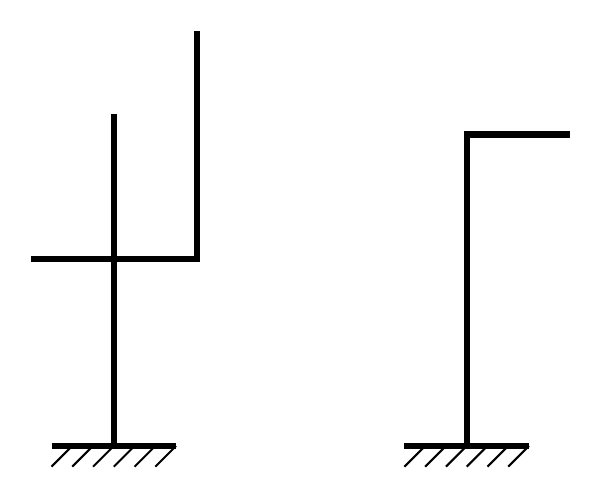
\begin{tikzpicture}[x=0.75pt,y=0.75pt,yscale=-1,xscale=1]
	%uncomment if require: \path (0,243); %set diagram left start at 0, and has height of 243
	
	%Straight Lines [id:da48723828101034194] 
	\draw [line width=2.25]    (210,210) -- (270,210) ;
	%Straight Lines [id:da9181027120373297] 
	\draw [line width=2.25]    (240,50) -- (240,210) ;
	%Straight Lines [id:da602622313919287] 
	\draw [line width=2.25]    (200,120) -- (280,120)-- (280,10) ;
	%Straight Lines [id:da9240962643084318] 
	\draw [line width=2.25]    (380,210) -- (440,210) ;
	%Straight Lines [id:da6088177156525376] 
	\draw [line width=2.25]    (410,210) -- (410,60)-- (460,60) ;
	%Straight Lines [id:da18772355497010085] 
	\draw    (230,210) -- (220,220) ;
	%Straight Lines [id:da4111734204635673] 
	\draw    (220,210) -- (210,220) ;
	%Straight Lines [id:da22170283469466634] 
	\draw    (250,210) -- (240,220) ;
	%Straight Lines [id:da37045531210319527] 
	\draw    (240,210) -- (230,220) ;
	%Straight Lines [id:da3409018442815923] 
	\draw    (270,210) -- (260,220) ;
	%Straight Lines [id:da5614281144127149] 
	\draw    (260,210) -- (250,220) ;
	%Straight Lines [id:da4814860558051475] 
	\draw    (400,210) -- (390,220) ;
	%Straight Lines [id:da24775805984689558] 
	\draw    (390,210) -- (380,220) ;
	%Straight Lines [id:da5468227638976404] 
	\draw    (420,210) -- (410,220) ;
	%Straight Lines [id:da8736964963523615] 
	\draw    (410,210) -- (400,220) ;
	%Straight Lines [id:da8905437847943618] 
	\draw    (440,210) -- (430,220) ;
	%Straight Lines [id:da39185002883344033] 
	\draw    (430,210) -- (420,220) ;
	
\end{tikzpicture}
\caption{第二条原则}
\end{figure}


\item 刚性节点看成3个约束,刚性封闭框格也看成3个约束。
\begin{figure}[!ht]
	\centering
\tikzset{every picture/.style={line width=0.75pt}} %set default line width to 0.75pt        

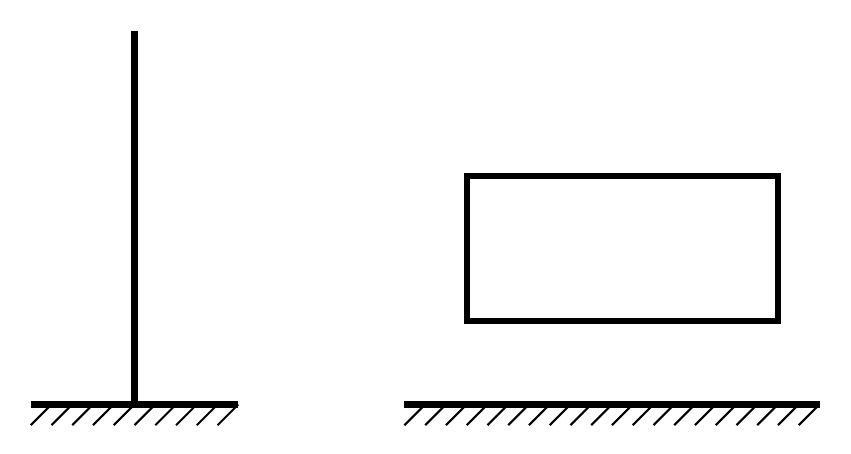
\begin{tikzpicture}[x=0.75pt,y=0.75pt,yscale=-1,xscale=1]
	%uncomment if require: \path (0,234); %set diagram left start at 0, and has height of 234
	
	%Straight Lines [id:da1494206630363457] 
	\draw [line width=2.25]    (140,200) -- (240,200) ;
	%Straight Lines [id:da021038683819858628] 
	\draw [line width=2.25]    (190,20) -- (190,200) ;
	%Straight Lines [id:da6437333320834968] 
	\draw    (140,210) -- (150,200) ;
	%Straight Lines [id:da04598717292338339] 
	\draw    (150,210) -- (160,200) ;
	%Straight Lines [id:da057725790041922576] 
	\draw    (160,210) -- (170,200) ;
	%Straight Lines [id:da12188365586198291] 
	\draw    (170,210) -- (180,200) ;
	%Straight Lines [id:da6384772771066007] 
	\draw    (180,210) -- (190,200) ;
	%Straight Lines [id:da6270858296097501] 
	\draw    (190,210) -- (200,200) ;
	%Straight Lines [id:da7291068701837558] 
	\draw    (200,210) -- (210,200) ;
	%Straight Lines [id:da9173213173554711] 
	\draw    (210,210) -- (220,200) ;
	%Straight Lines [id:da24059052404723258] 
	\draw    (220,210) -- (230,200) ;
	%Straight Lines [id:da33228461820253474] 
	\draw    (230,210) -- (240,200) ;
	%Straight Lines [id:da29709537451612844] 
	\draw [line width=2.25]    (320,200) -- (420,200) ;
	%Straight Lines [id:da01947431895506302] 
	\draw    (320,210) -- (330,200) ;
	%Straight Lines [id:da19400504371362426] 
	\draw    (330,210) -- (340,200) ;
	%Straight Lines [id:da5685365967757696] 
	\draw    (340,210) -- (350,200) ;
	%Straight Lines [id:da7406641383381025] 
	\draw    (350,210) -- (360,200) ;
	%Straight Lines [id:da8270353077372523] 
	\draw    (360,210) -- (370,200) ;
	%Straight Lines [id:da6479397769943023] 
	\draw    (370,210) -- (380,200) ;
	%Straight Lines [id:da49645436249634667] 
	\draw    (380,210) -- (390,200) ;
	%Straight Lines [id:da3702297825653882] 
	\draw    (390,210) -- (400,200) ;
	%Straight Lines [id:da17210221936369385] 
	\draw    (400,210) -- (410,200) ;
	%Straight Lines [id:da5254368727523482] 
	\draw    (410,210) -- (420,200) ;
	%Straight Lines [id:da6489335975911368] 
	\draw [line width=2.25]    (420,200) -- (520,200) ;
	%Straight Lines [id:da6011696339904511] 
	\draw    (420,210) -- (430,200) ;
	%Straight Lines [id:da3438004738519771] 
	\draw    (430,210) -- (440,200) ;
	%Straight Lines [id:da09185455292510825] 
	\draw    (440,210) -- (450,200) ;
	%Straight Lines [id:da436741128707431] 
	\draw    (450,210) -- (460,200) ;
	%Straight Lines [id:da17578128972263207] 
	\draw    (460,210) -- (470,200) ;
	%Straight Lines [id:da543290232241731] 
	\draw    (470,210) -- (480,200) ;
	%Straight Lines [id:da16264624135224204] 
	\draw    (480,210) -- (490,200) ;
	%Straight Lines [id:da5032217662761382] 
	\draw    (490,210) -- (500,200) ;
	%Straight Lines [id:da19134027955433153] 
	\draw    (500,210) -- (510,200) ;
	%Straight Lines [id:da5675548470527982] 
	\draw    (510,210) -- (520,200) ;
	%Shape: Rectangle [id:dp022641157747854024] 
	\draw  [line width=2.25]  (350,90) -- (500,90) -- (500,160) -- (350,160) -- cycle ;
	
	
\end{tikzpicture}
\caption{第三条原则}
\end{figure}


\item 一个铰接点看成两个约束。
\begin{figure}[!ht]
	\centering
\tikzset{every picture/.style={line width=0.75pt}} %set default line width to 0.75pt        

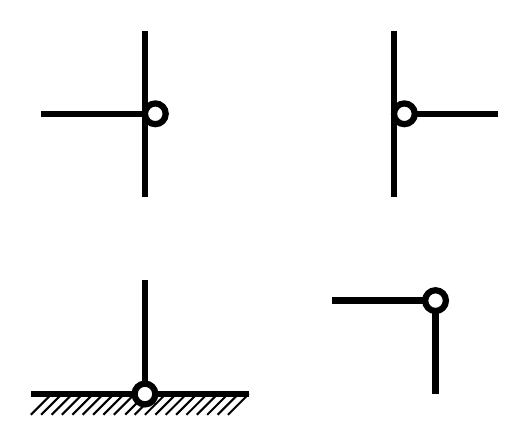
\begin{tikzpicture}[x=0.75pt,y=0.75pt,yscale=-1,xscale=1]
	%uncomment if require: \path (0,225); %set diagram left start at 0, and has height of 225
	
	%Straight Lines [id:da7495306508589998] 
	\draw [line width=2.25]    (250,15) -- (250,95) ;
	%Straight Lines [id:da0004590644200239691] 
	\draw [line width=2.25]    (200,55) -- (250,55) ;
	%Shape: Circle [id:dp27954834617974855] 
	\draw  [line width=2.25]  (250,55) .. controls (250,52.24) and (252.24,50) .. (255,50) .. controls (257.76,50) and (260,52.24) .. (260,55) .. controls (260,57.76) and (257.76,60) .. (255,60) .. controls (252.24,60) and (250,57.76) .. (250,55) -- cycle ;
	%Straight Lines [id:da43820486304875406] 
	\draw [line width=2.25]    (370,15) -- (370,95) ;
	%Shape: Circle [id:dp1653818479346405] 
	\draw  [line width=2.25]  (370,55) .. controls (370,52.24) and (372.24,50) .. (375,50) .. controls (377.76,50) and (380,52.24) .. (380,55) .. controls (380,57.76) and (377.76,60) .. (375,60) .. controls (372.24,60) and (370,57.76) .. (370,55) -- cycle ;
	%Straight Lines [id:da9474388544997172] 
	\draw [line width=2.25]    (380,55) -- (420,55) ;
	%Straight Lines [id:da8207995915439157] 
	\draw [line width=2.25]    (255,190) -- (300,190) ;
	%Straight Lines [id:da24832170430256295] 
	\draw [line width=2.25]    (250,135) -- (250,185) ;
	%Shape: Circle [id:dp950836324956635] 
	\draw  [line width=2.25]  (245,190) .. controls (245,187.24) and (247.24,185) .. (250,185) .. controls (252.76,185) and (255,187.24) .. (255,190) .. controls (255,192.76) and (252.76,195) .. (250,195) .. controls (247.24,195) and (245,192.76) .. (245,190) -- cycle ;
	%Straight Lines [id:da20767079793157217] 
	\draw [line width=2.25]    (195,190) -- (245,190) ;
	%Straight Lines [id:da67856168253064] 
	\draw    (205,190) -- (195,200) ;
	%Straight Lines [id:da8269844492241123] 
	\draw    (210,190) -- (200,200) ;
	%Straight Lines [id:da5520780633357969] 
	\draw    (215,190) -- (205,200) ;
	%Straight Lines [id:da3110548979040937] 
	\draw    (220,190) -- (210,200) ;
	%Straight Lines [id:da2437318948912921] 
	\draw    (225,190) -- (215,200) ;
	%Straight Lines [id:da16138152432547614] 
	\draw    (230,190) -- (220,200) ;
	%Straight Lines [id:da9976779088439263] 
	\draw    (235,190) -- (225,200) ;
	%Straight Lines [id:da2860931698295972] 
	\draw    (240,190) -- (230,200) ;
	%Straight Lines [id:da09703262828007042] 
	\draw    (245,190) -- (235,200) ;
	%Straight Lines [id:da9506295823364495] 
	\draw    (260,190) -- (250,200) ;
	%Straight Lines [id:da8289995329213529] 
	\draw    (265,190) -- (255,200) ;
	%Straight Lines [id:da9315047008315245] 
	\draw    (270,190) -- (260,200) ;
	%Straight Lines [id:da8689083923793353] 
	\draw    (275,190) -- (265,200) ;
	%Straight Lines [id:da9894480469151854] 
	\draw    (280,190) -- (270,200) ;
	%Straight Lines [id:da6030150323123316] 
	\draw    (285,190) -- (275,200) ;
	%Straight Lines [id:da5270374873518371] 
	\draw    (290,190) -- (280,200) ;
	%Straight Lines [id:da9828122738641056] 
	\draw    (295,190) -- (285,200) ;
	%Straight Lines [id:da9117856715321269] 
	\draw    (300,190) -- (290,200) ;
	%Straight Lines [id:da8886518239950592] 
	\draw [line width=2.25]    (340,145) -- (385,145) ;
	%Shape: Circle [id:dp7986495199828691] 
	\draw  [line width=2.25]  (385,145) .. controls (385,142.24) and (387.24,140) .. (390,140) .. controls (392.76,140) and (395,142.24) .. (395,145) .. controls (395,147.76) and (392.76,150) .. (390,150) .. controls (387.24,150) and (385,147.76) .. (385,145) -- cycle ;
	%Straight Lines [id:da3436002039309032] 
	\draw [line width=2.25]    (390,150) -- (390,190) ;
	%Straight Lines [id:da4255271061782404] 
	\draw    (250,195) -- (245,200) ;
	%Straight Lines [id:da09365524036838879] 
	\draw    (247.01,193.41) -- (240.51,199.91) ;
	
\end{tikzpicture}
\caption{第四条原则}
\end{figure}


\item $\displaystyle N$个连杆铰接,算$\displaystyle N-1$个铰接点。
\item 组合式铰链可以分解计算。
\begin{figure}[!ht]
	\centering
\tikzset{every picture/.style={line width=0.75pt}} %set default line width to 0.75pt        

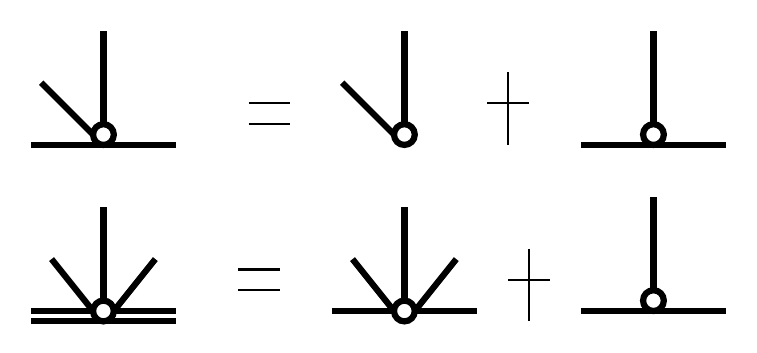
\begin{tikzpicture}[x=0.75pt,y=0.75pt,yscale=-1,xscale=1]
	%uncomment if require: \path (0,188); %set diagram left start at 0, and has height of 188
	
	%Straight Lines [id:da22317063315639074] 
	\draw [line width=2.25]    (160,75) -- (230,75) ;
	%Shape: Circle [id:dp9489222136216069] 
	\draw  [line width=2.25]  (190,70) .. controls (190,67.24) and (192.24,65) .. (195,65) .. controls (197.76,65) and (200,67.24) .. (200,70) .. controls (200,72.76) and (197.76,75) .. (195,75) .. controls (192.24,75) and (190,72.76) .. (190,70) -- cycle ;
	%Straight Lines [id:da20583145498241162] 
	\draw [line width=2.25]    (195,65) -- (195,20) ;
	%Straight Lines [id:da49673336594197814] 
	\draw [line width=2.25]    (165,45) -- (190,70) ;
	%Straight Lines [id:da285413877471715] 
	\draw    (265,55) -- (285,55) ;
	%Straight Lines [id:da8188364451016874] 
	\draw    (265,65) -- (285,65) ;
	%Shape: Circle [id:dp653456399289231] 
	\draw  [line width=2.25]  (335,70) .. controls (335,67.24) and (337.24,65) .. (340,65) .. controls (342.76,65) and (345,67.24) .. (345,70) .. controls (345,72.76) and (342.76,75) .. (340,75) .. controls (337.24,75) and (335,72.76) .. (335,70) -- cycle ;
	%Straight Lines [id:da9728875511808333] 
	\draw [line width=2.25]    (340,65) -- (340,20) ;
	%Straight Lines [id:da5379619411836745] 
	\draw [line width=2.25]    (310,45) -- (335,70) ;
	%Straight Lines [id:da990059257334768] 
	\draw    (380,55) -- (400,55) ;
	%Straight Lines [id:da5129400373430522] 
	\draw    (390,40) -- (390,75) ;
	%Straight Lines [id:da9355451773133447] 
	\draw [line width=2.25]    (425,75) -- (495,75) ;
	%Shape: Circle [id:dp11432021175312213] 
	\draw  [line width=2.25]  (455,70) .. controls (455,67.24) and (457.24,65) .. (460,65) .. controls (462.76,65) and (465,67.24) .. (465,70) .. controls (465,72.76) and (462.76,75) .. (460,75) .. controls (457.24,75) and (455,72.76) .. (455,70) -- cycle ;
	%Straight Lines [id:da8859230358800001] 
	\draw [line width=2.25]    (460,65) -- (460,20) ;
	%Straight Lines [id:da31215157818751194] 
	\draw [line width=2.25]    (160,160) -- (230,160) ;
	%Shape: Circle [id:dp5808272231115363] 
	\draw  [line width=2.25]  (190,155) .. controls (190,152.24) and (192.24,150) .. (195,150) .. controls (197.76,150) and (200,152.24) .. (200,155) .. controls (200,157.76) and (197.76,160) .. (195,160) .. controls (192.24,160) and (190,157.76) .. (190,155) -- cycle ;
	%Straight Lines [id:da6298355434059231] 
	\draw [line width=2.25]    (195,150) -- (195,105) ;
	%Straight Lines [id:da8001944987706804] 
	\draw [line width=2.25]    (170,130) -- (190,155) ;
	%Straight Lines [id:da5246616482260829] 
	\draw [line width=2.25]    (160,155) -- (190,155) ;
	%Straight Lines [id:da2919646235467013] 
	\draw [line width=2.25]    (200,155) -- (230,155) ;
	%Straight Lines [id:da2400442486059513] 
	\draw [line width=2.25]    (200,155) -- (220,130) ;
	%Straight Lines [id:da6721942655766391] 
	\draw    (260,135) -- (280,135) ;
	%Straight Lines [id:da4448569884443778] 
	\draw    (260,145) -- (280,145) ;
	%Shape: Circle [id:dp36494815010853787] 
	\draw  [line width=2.25]  (335,155) .. controls (335,152.24) and (337.24,150) .. (340,150) .. controls (342.76,150) and (345,152.24) .. (345,155) .. controls (345,157.76) and (342.76,160) .. (340,160) .. controls (337.24,160) and (335,157.76) .. (335,155) -- cycle ;
	%Straight Lines [id:da5657859649112764] 
	\draw [line width=2.25]    (340,150) -- (340,105) ;
	%Straight Lines [id:da5555589513444292] 
	\draw [line width=2.25]    (315,130) -- (335,155) ;
	%Straight Lines [id:da06438649379908123] 
	\draw [line width=2.25]    (305,155) -- (335,155) ;
	%Straight Lines [id:da6627977154856652] 
	\draw [line width=2.25]    (345,155) -- (375,155) ;
	%Straight Lines [id:da9999680845849797] 
	\draw [line width=2.25]    (345,155) -- (365,130) ;
	%Straight Lines [id:da8827320005031338] 
	\draw [line width=2.25]    (425,155) -- (495,155) ;
	%Shape: Circle [id:dp7062653938850874] 
	\draw  [line width=2.25]  (455,150) .. controls (455,147.24) and (457.24,145) .. (460,145) .. controls (462.76,145) and (465,147.24) .. (465,150) .. controls (465,152.76) and (462.76,155) .. (460,155) .. controls (457.24,155) and (455,152.76) .. (455,150) -- cycle ;
	%Straight Lines [id:da3725659895410498] 
	\draw [line width=2.25]    (460,145) -- (460,100) ;
	%Straight Lines [id:da41287463765411303] 
	\draw    (390,140) -- (410,140) ;
	%Straight Lines [id:da6770309244838046] 
	\draw    (400,125) -- (400,160) ;
	
\end{tikzpicture}
\caption{第六条原则}
\end{figure}
 \end{enumerate}

\section{计算规则}
\begin{enumerate}
\item 分析有几个独立杆件,按照原则2判定;

\item 计算独立的杆件有几根,乘3就是静定所需的约束数;

\item 计算杆件和地面的独立刚节点,乘3就是约束数;计算独立杆件和地面的铰接点,乘2就是约束数;如果有刚性封闭框格,乘3就是约束数;

\item 约束数减去静定约束数量就是超静定次数;
\end{enumerate}
\section{计算讲解}
\begin{enumerate}
	\item 
	\begin{figure}[!ht]
		\centering
\tikzset{every picture/.style={line width=0.75pt}} %set default line width to 0.75pt        

\begin{tikzpicture}[x=0.75pt,y=0.75pt,yscale=-1,xscale=1]
	%uncomment if require: \path (0,150); %set diagram left start at 0, and has height of 150
	
	%Shape: Circle [id:dp9914182276372867] 
	\draw  [line width=2.25]  (185,40) .. controls (185,37.24) and (187.24,35) .. (190,35) .. controls (192.76,35) and (195,37.24) .. (195,40) .. controls (195,42.76) and (192.76,45) .. (190,45) .. controls (187.24,45) and (185,42.76) .. (185,40) -- cycle ;
	%Shape: Circle [id:dp8016647757210809] 
	\draw  [line width=2.25]  (215,40) .. controls (215,37.24) and (217.24,35) .. (220,35) .. controls (222.76,35) and (225,37.24) .. (225,40) .. controls (225,42.76) and (222.76,45) .. (220,45) .. controls (217.24,45) and (215,42.76) .. (215,40) -- cycle ;
	%Straight Lines [id:da18362914864003743] 
	\draw [line width=2.25]    (170,40) -- (185,40) ;
	%Straight Lines [id:da4933046172461768] 
	\draw [line width=2.25]    (195,40) -- (215,40) ;
	%Straight Lines [id:da2711141890639779] 
	\draw [line width=2.25]    (225,40) -- (240,40) ;
	%Straight Lines [id:da32562115568615746] 
	\draw [line width=2.25]    (202.11,19.09) -- (192.51,35.49) ;
	%Shape: Circle [id:dp10414866216305319] 
	\draw  [line width=2.25]  (200,15) .. controls (200,12.24) and (202.24,10) .. (205,10) .. controls (207.76,10) and (210,12.24) .. (210,15) .. controls (210,17.76) and (207.76,20) .. (205,20) .. controls (202.24,20) and (200,17.76) .. (200,15) -- cycle ;
	%Straight Lines [id:da5873683565737926] 
	\draw [line width=2.25]    (207.31,18.69) -- (216.91,35.49) ;
	%Straight Lines [id:da6122438296070845] 
	\draw [line width=2.25]    (210,15) -- (340,15) ;
	%Shape: Circle [id:dp998731562932277] 
	\draw  [line width=2.25]  (340,15) .. controls (340,12.24) and (342.24,10) .. (345,10) .. controls (347.76,10) and (350,12.24) .. (350,15) .. controls (350,17.76) and (347.76,20) .. (345,20) .. controls (342.24,20) and (340,17.76) .. (340,15) -- cycle ;
	%Straight Lines [id:da285750534125607] 
	\draw [line width=2.25]    (345,20) -- (345,35) ;
	%Shape: Circle [id:dp8643094970594003] 
	\draw  [line width=2.25]  (340,40) .. controls (340,37.24) and (342.24,35) .. (345,35) .. controls (347.76,35) and (350,37.24) .. (350,40) .. controls (350,42.76) and (347.76,45) .. (345,45) .. controls (342.24,45) and (340,42.76) .. (340,40) -- cycle ;
	%Straight Lines [id:da013884097629328185] 
	\draw [line width=2.25]    (350,40) -- (370,40) ;
	%Straight Lines [id:da4379233825227673] 
	\draw [line width=2.25]    (320,40) -- (340,40) ;
	%Straight Lines [id:da050331560047672586] 
	\draw    (175,40) -- (170,45) ;
	%Straight Lines [id:da5517772901304674] 
	\draw    (180,40) -- (175,45) ;
	%Straight Lines [id:da316868350624264] 
	\draw    (185,40) -- (180,45) ;
	%Straight Lines [id:da0055372853104704856] 
	\draw    (200,40) -- (195,45) ;
	%Straight Lines [id:da9878254867743188] 
	\draw    (205,40) -- (200,45) ;
	%Straight Lines [id:da9680340560547118] 
	\draw    (210,40) -- (205,45) ;
	%Straight Lines [id:da34070066708396585] 
	\draw    (215,40) -- (210,45) ;
	%Straight Lines [id:da6403315980082345] 
	\draw    (230,40) -- (225,45) ;
	%Straight Lines [id:da321219972932689] 
	\draw    (235,40) -- (230,45) ;
	%Straight Lines [id:da7995635215222967] 
	\draw    (240,40) -- (235,45) ;
	%Straight Lines [id:da9215992744839685] 
	\draw    (325,40) -- (320,45) ;
	%Straight Lines [id:da2812531761231982] 
	\draw    (330,40) -- (325,45) ;
	%Straight Lines [id:da4032182147598755] 
	\draw    (335,40) -- (330,45) ;
	%Straight Lines [id:da6243992642409588] 
	\draw    (340,40) -- (335,45) ;
	%Straight Lines [id:da6384236910934022] 
	\draw    (355,40) -- (350,45) ;
	%Straight Lines [id:da5327993153676476] 
	\draw    (360,40) -- (355,45) ;
	%Straight Lines [id:da8493258949179276] 
	\draw    (365,40) -- (360,45) ;
	%Straight Lines [id:da07197380753727045] 
	\draw    (370,40) -- (365,45) ;
	%Shape: Circle [id:dp6897680758787883] 
	\draw  [line width=2.25]  (185,105) .. controls (185,102.24) and (187.24,100) .. (190,100) .. controls (192.76,100) and (195,102.24) .. (195,105) .. controls (195,107.76) and (192.76,110) .. (190,110) .. controls (187.24,110) and (185,107.76) .. (185,105) -- cycle ;
	%Shape: Circle [id:dp42195267814734905] 
	\draw  [line width=2.25]  (215,105) .. controls (215,102.24) and (217.24,100) .. (220,100) .. controls (222.76,100) and (225,102.24) .. (225,105) .. controls (225,107.76) and (222.76,110) .. (220,110) .. controls (217.24,110) and (215,107.76) .. (215,105) -- cycle ;
	%Straight Lines [id:da6902342346200661] 
	\draw [line width=2.25]    (170,105) -- (185,105) ;
	%Straight Lines [id:da9657095873534995] 
	\draw [line width=2.25]    (195,105) -- (215,105) ;
	%Straight Lines [id:da2165486146188269] 
	\draw [line width=2.25]    (225,105) -- (240,105) ;
	%Straight Lines [id:da10339878228696708] 
	\draw [line width=2.25]    (202.11,84.09) -- (192.51,100.49) ;
	%Shape: Circle [id:dp9909002560822875] 
	\draw  [line width=2.25]  (200,80) .. controls (200,77.24) and (202.24,75) .. (205,75) .. controls (207.76,75) and (210,77.24) .. (210,80) .. controls (210,82.76) and (207.76,85) .. (205,85) .. controls (202.24,85) and (200,82.76) .. (200,80) -- cycle ;
	%Straight Lines [id:da8879342100630068] 
	\draw [line width=2.25]    (207.31,83.69) -- (216.91,100.49) ;
	%Straight Lines [id:da3927764270501517] 
	\draw [line width=2.25]    (210,80) -- (340,80) ;
	%Shape: Circle [id:dp6732081377782273] 
	\draw  [line width=2.25]  (340,80) .. controls (340,77.24) and (342.24,75) .. (345,75) .. controls (347.76,75) and (350,77.24) .. (350,80) .. controls (350,82.76) and (347.76,85) .. (345,85) .. controls (342.24,85) and (340,82.76) .. (340,80) -- cycle ;
	%Straight Lines [id:da3628372644182305] 
	\draw [line width=2.25]    (345,85) -- (345,100) ;
	%Shape: Circle [id:dp01818429868303073] 
	\draw  [line width=2.25]  (340,105) .. controls (340,102.24) and (342.24,100) .. (345,100) .. controls (347.76,100) and (350,102.24) .. (350,105) .. controls (350,107.76) and (347.76,110) .. (345,110) .. controls (342.24,110) and (340,107.76) .. (340,105) -- cycle ;
	%Straight Lines [id:da26581419831396746] 
	\draw [line width=2.25]    (350,105) -- (370,105) ;
	%Straight Lines [id:da37792553011290275] 
	\draw [line width=2.25]    (320,105) -- (340,105) ;
	%Straight Lines [id:da21034468031376785] 
	\draw    (175,105) -- (170,110) ;
	%Straight Lines [id:da1437802844020426] 
	\draw    (180,105) -- (175,110) ;
	%Straight Lines [id:da7661815682433819] 
	\draw    (185,105) -- (180,110) ;
	%Straight Lines [id:da736235423281284] 
	\draw    (200,105) -- (195,110) ;
	%Straight Lines [id:da2708379314427376] 
	\draw    (205,105) -- (200,110) ;
	%Straight Lines [id:da11525260129749548] 
	\draw    (210,105) -- (205,110) ;
	%Straight Lines [id:da09009400744407436] 
	\draw    (215,105) -- (210,110) ;
	%Straight Lines [id:da49628465884200734] 
	\draw    (230,105) -- (225,110) ;
	%Straight Lines [id:da061512995343041554] 
	\draw    (235,105) -- (230,110) ;
	%Straight Lines [id:da6359910752574212] 
	\draw    (240,105) -- (235,110) ;
	%Straight Lines [id:da5273528296671772] 
	\draw    (325,105) -- (320,110) ;
	%Straight Lines [id:da21285129509789935] 
	\draw    (330,105) -- (325,110) ;
	%Straight Lines [id:da3339925878629304] 
	\draw    (335,105) -- (330,110) ;
	%Straight Lines [id:da3261037098825197] 
	\draw    (340,105) -- (335,110) ;
	%Straight Lines [id:da38906066370412895] 
	\draw    (355,105) -- (350,110) ;
	%Straight Lines [id:da50648220688569] 
	\draw    (360,105) -- (355,110) ;
	%Straight Lines [id:da4506439647752649] 
	\draw    (365,105) -- (360,110) ;
	%Straight Lines [id:da8329875654515277] 
	\draw    (370,105) -- (365,110) ;
	
	% Text Node
	\draw (175,87) node [anchor=north west][inner sep=0.75pt]  [font=\fontsize{0.53em}{0.64em}\selectfont] [align=left] {杆1};
	% Text Node
	\draw (216,87) node [anchor=north west][inner sep=0.75pt]  [font=\fontsize{0.53em}{0.64em}\selectfont] [align=left] {杆1};
	% Text Node
	\draw (266,68) node [anchor=north west][inner sep=0.75pt]  [font=\fontsize{0.53em}{0.64em}\selectfont] [align=left] {杆1};
	% Text Node
	\draw (347,88) node [anchor=north west][inner sep=0.75pt]  [font=\fontsize{0.53em}{0.64em}\selectfont] [align=left] {杆1};
	% Text Node
	\draw (201,63) node [anchor=north west][inner sep=0.75pt]  [font=\fontsize{0.53em}{0.64em}\selectfont] [align=left] {铰2};
	% Text Node
	\draw (182,113) node [anchor=north west][inner sep=0.75pt]  [font=\fontsize{0.53em}{0.64em}\selectfont] [align=left] {铰1};
	% Text Node
	\draw (212,113) node [anchor=north west][inner sep=0.75pt]  [font=\fontsize{0.53em}{0.64em}\selectfont] [align=left] {铰1};
	% Text Node
	\draw (336,63) node [anchor=north west][inner sep=0.75pt]  [font=\fontsize{0.53em}{0.64em}\selectfont] [align=left] {铰1};
	% Text Node
	\draw (337,113) node [anchor=north west][inner sep=0.75pt]  [font=\fontsize{0.53em}{0.64em}\selectfont] [align=left] {铰1};
	
\end{tikzpicture}
\caption{题图1}
\end{figure}
4根杆件,需要$\displaystyle 3\times 4=12$个约束;6个铰,共$\displaystyle 6\times 2=12$个约束,静定。

\item 
\begin{figure}[!ht]
	\centering
\tikzset{every picture/.style={line width=0.75pt}} %set default line width to 0.75pt        

\begin{tikzpicture}[x=0.75pt,y=0.75pt,yscale=-1,xscale=1]
	%uncomment if require: \path (0,300); %set diagram left start at 0, and has height of 300
	
	%Straight Lines [id:da7637584054348636] 
	\draw [line width=2.25]    (114,155) -- (114,170) ;
	%Shape: Circle [id:dp7403286552960038] 
	\draw  [line width=2.25]  (109,175) .. controls (109,172.24) and (111.24,170) .. (114,170) .. controls (116.76,170) and (119,172.24) .. (119,175) .. controls (119,177.76) and (116.76,180) .. (114,180) .. controls (111.24,180) and (109,177.76) .. (109,175) -- cycle ;
	%Straight Lines [id:da5534934091686219] 
	\draw [line width=2.25]    (114,180) -- (114,195) ;
	%Straight Lines [id:da8562095168105262] 
	\draw [line width=2.25]    (119,175) -- (134,175) ;
	%Shape: Circle [id:dp3019921419913527] 
	\draw  [line width=2.25]  (134,175) .. controls (134,172.24) and (136.24,170) .. (139,170) .. controls (141.76,170) and (144,172.24) .. (144,175) .. controls (144,177.76) and (141.76,180) .. (139,180) .. controls (136.24,180) and (134,177.76) .. (134,175) -- cycle ;
	%Straight Lines [id:da7424238245600134] 
	\draw [line width=2.25]    (139,180) -- (139,195) ;
	%Shape: Circle [id:dp6493364599828684] 
	\draw  [line width=2.25]  (134,200) .. controls (134,197.24) and (136.24,195) .. (139,195) .. controls (141.76,195) and (144,197.24) .. (144,200) .. controls (144,202.76) and (141.76,205) .. (139,205) .. controls (136.24,205) and (134,202.76) .. (134,200) -- cycle ;
	%Straight Lines [id:da04749018352898071] 
	\draw [line width=2.25]    (134,200) -- (119,200) ;
	%Straight Lines [id:da079002228020574] 
	\draw [line width=2.25]    (144,200) -- (159,200) ;
	%Straight Lines [id:da7461781062527937] 
	\draw [line width=2.25]    (139,170) -- (139,100)--(164,80) ;
	%Shape: Circle [id:dp07267328808005824] 
	\draw  [line width=2.25]  (164,80) .. controls (164,77.24) and (166.24,75) .. (169,75) .. controls (171.76,75) and (174,77.24) .. (174,80) .. controls (174,82.76) and (171.76,85) .. (169,85) .. controls (166.24,85) and (164,82.76) .. (164,80) -- cycle ;
	%Straight Lines [id:da009934043155127359] 
	\draw [line width=2.25]    (164,175) -- (184,175) ;
	%Straight Lines [id:da61956142167679] 
	\draw [line width=2.25]    (189.68,49.41)--(174,60) -- (174,175) ;
	%Shape: Circle [id:dp4597205490392009] 
	\draw  [line width=2.25]  (189.5,48) .. controls (189.5,45.24) and (191.74,43) .. (194.5,43) .. controls (197.26,43) and (199.5,45.24) .. (199.5,48) .. controls (199.5,50.76) and (197.26,53) .. (194.5,53) .. controls (191.74,53) and (189.5,50.76) .. (189.5,48) -- cycle ;
	%Straight Lines [id:da1070988873213643] 
	\draw [line width=2.25]    (198.68,45.08) -- (219,30) ;
	%Shape: Circle [id:dp8488215887475352] 
	\draw  [line width=2.25]  (218,27.67) .. controls (218,24.91) and (220.24,22.67) .. (223,22.67) .. controls (225.76,22.67) and (228,24.91) .. (228,27.67) .. controls (228,30.43) and (225.76,32.67) .. (223,32.67) .. controls (220.24,32.67) and (218,30.43) .. (218,27.67) -- cycle ;
	%Straight Lines [id:da48607158786038873] 
	\draw [line width=2.25]    (227,24) -- (254,5)-- (254,175) ;
	%Straight Lines [id:da6423924781209616] 
	\draw [line width=2.25]    (239,175) -- (269,175) ;
	%Straight Lines [id:da08639987813390859] 
	\draw    (109,160) -- (114,155) ;
	%Straight Lines [id:da45610594225215273] 
	\draw    (109,165) -- (114,160) ;
	%Straight Lines [id:da08803307470646748] 
	\draw    (109,170) -- (114,165) ;
	%Straight Lines [id:da5120222574356765] 
	\draw    (109,185) -- (114,180) ;
	%Straight Lines [id:da32590875409421227] 
	\draw    (109,190) -- (114,185) ;
	%Straight Lines [id:da8866333093245795] 
	\draw    (109,195) -- (114,190) ;
	%Straight Lines [id:da2980534124119898] 
	\draw    (119,205) -- (124,200) ;
	%Straight Lines [id:da19034693528208213] 
	\draw    (124,205) -- (129,200) ;
	%Straight Lines [id:da8321953875333166] 
	\draw    (129,205) -- (134,200) ;
	%Straight Lines [id:da8458660783523986] 
	\draw    (144,205) -- (149,200) ;
	%Straight Lines [id:da6127450746298369] 
	\draw    (149,205) -- (154,200) ;
	%Straight Lines [id:da4076568055341101] 
	\draw    (154,205) -- (159,200) ;
	%Straight Lines [id:da7888445806501094] 
	\draw    (164,180) -- (169,175) ;
	%Straight Lines [id:da30866939107003155] 
	\draw    (169,180) -- (174,175) ;
	%Straight Lines [id:da6933505928000521] 
	\draw    (174,180) -- (179,175) ;
	%Straight Lines [id:da4334051416688147] 
	\draw    (179,180) -- (184,175) ;
	%Straight Lines [id:da18248568787536756] 
	\draw    (239,180) -- (244,175) ;
	%Straight Lines [id:da2771412338867738] 
	\draw    (244,180) -- (249,175) ;
	%Straight Lines [id:da8778566418265144] 
	\draw    (249,180) -- (254,175) ;
	%Straight Lines [id:da4738801319278658] 
	\draw    (254,180) -- (259,175) ;
	%Straight Lines [id:da9454711411394303] 
	\draw    (259,180) -- (264,175) ;
	%Straight Lines [id:da5450482155303857] 
	\draw    (264,180) -- (269,175) ;
	%Straight Lines [id:da054873388327274064] 
	\draw [line width=2.25]    (364,155) -- (364,170) ;
	%Shape: Circle [id:dp24716371333640286] 
	\draw  [line width=2.25]  (359,175) .. controls (359,172.24) and (361.24,170) .. (364,170) .. controls (366.76,170) and (369,172.24) .. (369,175) .. controls (369,177.76) and (366.76,180) .. (364,180) .. controls (361.24,180) and (359,177.76) .. (359,175) -- cycle ;
	%Straight Lines [id:da43651764046393016] 
	\draw [line width=2.25]    (364,180) -- (364,195) ;
	%Straight Lines [id:da2376794126487809] 
	\draw [line width=2.25]    (369,175) -- (384,175) ;
	%Shape: Circle [id:dp12850278034368912] 
	\draw  [line width=2.25]  (384,175) .. controls (384,172.24) and (386.24,170) .. (389,170) .. controls (391.76,170) and (394,172.24) .. (394,175) .. controls (394,177.76) and (391.76,180) .. (389,180) .. controls (386.24,180) and (384,177.76) .. (384,175) -- cycle ;
	%Straight Lines [id:da7776740617858564] 
	\draw [line width=2.25]    (389,180) -- (389,195) ;
	%Shape: Circle [id:dp7177595274102815] 
	\draw  [line width=2.25]  (384,200) .. controls (384,197.24) and (386.24,195) .. (389,195) .. controls (391.76,195) and (394,197.24) .. (394,200) .. controls (394,202.76) and (391.76,205) .. (389,205) .. controls (386.24,205) and (384,202.76) .. (384,200) -- cycle ;
	%Straight Lines [id:da6987814615892838] 
	\draw [line width=2.25]    (384,200) -- (369,200) ;
	%Straight Lines [id:da08474458052218026] 
	\draw [line width=2.25]    (394,200) -- (409,200) ;
	%Straight Lines [id:da12026044428732141] 
	\draw [color={rgb, 255:red, 208; green, 2; blue, 27 }  ,draw opacity=1 ][line width=2.25]    (389,170) -- (389,100)-- (414,80) ;
	%Shape: Circle [id:dp8560318738218973] 
	\draw  [line width=2.25]  (414,80) .. controls (414,77.24) and (416.24,75) .. (419,75) .. controls (421.76,75) and (424,77.24) .. (424,80) .. controls (424,82.76) and (421.76,85) .. (419,85) .. controls (416.24,85) and (414,82.76) .. (414,80) -- cycle ;
	%Straight Lines [id:da8514782283464049] 
	\draw [line width=2.25]    (414,175) -- (434,175) ;
	%Straight Lines [id:da9312876373119325] 
	\draw [color={rgb, 255:red, 245; green, 166; blue, 35 }  ,draw opacity=1 ][line width=2.25]    (439.67,49.33)--(424,60) -- (424,175) ;
	%Shape: Circle [id:dp12837891653420574] 
	\draw  [line width=2.25]  (439.5,48) .. controls (439.5,45.24) and (441.74,43) .. (444.5,43) .. controls (447.26,43) and (449.5,45.24) .. (449.5,48) .. controls (449.5,50.76) and (447.26,53) .. (444.5,53) .. controls (441.74,53) and (439.5,50.76) .. (439.5,48) -- cycle ;
	%Straight Lines [id:da6063270705374815] 
	\draw [line width=2.25]    (448.68,45.08) -- (469,30) ;
	%Shape: Circle [id:dp6887941414929426] 
	\draw  [line width=2.25]  (468,27.67) .. controls (468,24.91) and (470.24,22.67) .. (473,22.67) .. controls (475.76,22.67) and (478,24.91) .. (478,27.67) .. controls (478,30.43) and (475.76,32.67) .. (473,32.67) .. controls (470.24,32.67) and (468,30.43) .. (468,27.67) -- cycle ;
	%Straight Lines [id:da9292587966472341] 
	\draw [color={rgb, 255:red, 74; green, 144; blue, 226 }  ,draw opacity=1 ][line width=2.25]    (477,24) -- (504,5)-- (504,175) ;
	%Straight Lines [id:da28067516290507477] 
	\draw [line width=2.25]    (489,175) -- (519,175) ;
	%Straight Lines [id:da891778097992113] 
	\draw    (359,160) -- (364,155) ;
	%Straight Lines [id:da7063785899748167] 
	\draw    (359,165) -- (364,160) ;
	%Straight Lines [id:da25053466145898295] 
	\draw    (359,170) -- (364,165) ;
	%Straight Lines [id:da7995502019059022] 
	\draw    (359,185) -- (364,180) ;
	%Straight Lines [id:da9831226426794244] 
	\draw    (359,190) -- (364,185) ;
	%Straight Lines [id:da18415416411539143] 
	\draw    (359,195) -- (364,190) ;
	%Straight Lines [id:da9761220428228994] 
	\draw    (369,205) -- (374,200) ;
	%Straight Lines [id:da40051814183181245] 
	\draw    (374,205) -- (379,200) ;
	%Straight Lines [id:da8831891405636185] 
	\draw    (379,205) -- (384,200) ;
	%Straight Lines [id:da8411012085905389] 
	\draw    (394,205) -- (399,200) ;
	%Straight Lines [id:da200790702061715] 
	\draw    (399,205) -- (404,200) ;
	%Straight Lines [id:da6129628031322918] 
	\draw    (404,205) -- (409,200) ;
	%Straight Lines [id:da7353173586046777] 
	\draw    (414,180) -- (419,175) ;
	%Straight Lines [id:da9904540615836375] 
	\draw    (419,180) -- (424,175) ;
	%Straight Lines [id:da7318069911056322] 
	\draw    (424,180) -- (429,175) ;
	%Straight Lines [id:da32391179548374627] 
	\draw    (429,180) -- (434,175) ;
	%Straight Lines [id:da4608611596174381] 
	\draw    (489,180) -- (494,175) ;
	%Straight Lines [id:da6923979028687459] 
	\draw    (494,180) -- (499,175) ;
	%Straight Lines [id:da3047112872517306] 
	\draw    (499,180) -- (504,175) ;
	%Straight Lines [id:da9918481123910363] 
	\draw    (504,180) -- (509,175) ;
	%Straight Lines [id:da9179836925630867] 
	\draw    (509,180) -- (514,175) ;
	%Straight Lines [id:da9108078478666357] 
	\draw    (514,180) -- (519,175) ;
	
	% Text Node
	\draw (340,167) node [anchor=north west][inner sep=0.75pt]   [align=left] {{\fontsize{0.53em}{0.64em}\selectfont 1铰}};
	% Text Node
	\draw (381,208) node [anchor=north west][inner sep=0.75pt]   [align=left] {{\fontsize{0.53em}{0.64em}\selectfont 1铰}};
	% Text Node
	\draw (425,72) node [anchor=north west][inner sep=0.75pt]   [align=left] {{\fontsize{0.53em}{0.64em}\selectfont 1铰}};
	% Text Node
	\draw (441.67,52.33) node [anchor=north west][inner sep=0.75pt]   [align=left] {{\fontsize{0.53em}{0.64em}\selectfont 1铰}};
	% Text Node
	\draw (470,32) node [anchor=north west][inner sep=0.75pt]   [align=left] {{\fontsize{0.53em}{0.64em}\selectfont 1铰}};
	% Text Node
	\draw (395,157) node [anchor=north west][inner sep=0.75pt]   [align=left] {{\fontsize{0.53em}{0.64em}\selectfont 2铰}};
	% Text Node
	\draw (370,157) node [anchor=north west][inner sep=0.75pt]   [align=left] {{\fontsize{0.53em}{0.64em}\selectfont 1杆}};
	% Text Node
	\draw (391,178) node [anchor=north west][inner sep=0.75pt]   [align=left] {{\fontsize{0.53em}{0.64em}\selectfont 1杆}};
	% Text Node
	\draw (370,122) node [anchor=north west][inner sep=0.75pt]   [align=left] {{\fontsize{0.53em}{0.64em}\selectfont 1杆}};
	% Text Node
	\draw (425,122) node [anchor=north west][inner sep=0.75pt]   [align=left] {{\fontsize{0.53em}{0.64em}\selectfont 1杆}};
	% Text Node
	\draw (505,107) node [anchor=north west][inner sep=0.75pt]   [align=left] {{\fontsize{0.53em}{0.64em}\selectfont 1杆}};
	% Text Node
	\draw (450,22) node [anchor=north west][inner sep=0.75pt]   [align=left] {{\fontsize{0.53em}{0.64em}\selectfont 1杆}};
	
	
\end{tikzpicture}
\caption{题图2}
\end{figure}
6根杆,需要18个静定约束;7个铰链,两个刚性节点,共20个约束,所以静不定。

\item 
\begin{figure}[!ht]
	\centering
\tikzset{every picture/.style={line width=0.75pt}} %set default line width to 0.75pt        

\begin{tikzpicture}[x=0.75pt,y=0.75pt,yscale=-1,xscale=1]
	%uncomment if require: \path (0,236); %set diagram left start at 0, and has height of 236
	
	%Shape: Circle [id:dp23519565043611412] 
	\draw  [line width=2.25]  (200,70) .. controls (200,67.24) and (202.24,65) .. (205,65) .. controls (207.76,65) and (210,67.24) .. (210,70) .. controls (210,72.76) and (207.76,75) .. (205,75) .. controls (202.24,75) and (200,72.76) .. (200,70) -- cycle ;
	%Straight Lines [id:da46219693531366635] 
	\draw [line width=2.25]    (200,70) -- (185,70) ;
	%Straight Lines [id:da594407196827959] 
	\draw [line width=2.25]    (205,75) -- (205,90) ;
	%Straight Lines [id:da2623331199355414] 
	\draw [line width=2.25]    (210,95) -- (225,95) ;
	%Shape: Circle [id:dp3367897921131897] 
	\draw  [line width=2.25]  (175,70) .. controls (175,67.24) and (177.24,65) .. (180,65) .. controls (182.76,65) and (185,67.24) .. (185,70) .. controls (185,72.76) and (182.76,75) .. (180,75) .. controls (177.24,75) and (175,72.76) .. (175,70) -- cycle ;
	%Shape: Circle [id:dp0264178961039494] 
	\draw  [line width=2.25]  (200,95) .. controls (200,92.24) and (202.24,90) .. (205,90) .. controls (207.76,90) and (210,92.24) .. (210,95) .. controls (210,97.76) and (207.76,100) .. (205,100) .. controls (202.24,100) and (200,97.76) .. (200,95) -- cycle ;
	%Straight Lines [id:da8609459024119492] 
	\draw [line width=2.25]    (185,95) -- (200,95) ;
	%Straight Lines [id:da5410908699076704] 
	\draw [line width=2.25]    (180,50) -- (180,65) ;
	%Straight Lines [id:da15337381161283403] 
	\draw [line width=2.25]    (180,75) -- (180,90) ;
	%Straight Lines [id:da2922082483040842] 
	\draw [line width=2.25]    (210,70) -- (280,70) ;
	%Shape: Circle [id:dp12119416785575376] 
	\draw  [line width=2.25]  (280,70) .. controls (280,67.24) and (282.24,65) .. (285,65) .. controls (287.76,65) and (290,67.24) .. (290,70) .. controls (290,72.76) and (287.76,75) .. (285,75) .. controls (282.24,75) and (280,72.76) .. (280,70) -- cycle ;
	%Straight Lines [id:da6006693672681356] 
	\draw [line width=2.25]    (205,65) -- (205,35) ;
	%Shape: Circle [id:dp23991289892963974] 
	\draw  [line width=2.25]  (200,30) .. controls (200,27.24) and (202.24,25) .. (205,25) .. controls (207.76,25) and (210,27.24) .. (210,30) .. controls (210,32.76) and (207.76,35) .. (205,35) .. controls (202.24,35) and (200,32.76) .. (200,30) -- cycle ;
	%Straight Lines [id:da25189205157242567] 
	\draw [line width=2.25]    (210,30) -- (280,30) ;
	%Straight Lines [id:da4458092198057997] 
	\draw [line width=2.25]    (285,65) -- (285,35) ;
	%Shape: Circle [id:dp8272442420888615] 
	\draw  [line width=2.25]  (280,30) .. controls (280,27.24) and (282.24,25) .. (285,25) .. controls (287.76,25) and (290,27.24) .. (290,30) .. controls (290,32.76) and (287.76,35) .. (285,35) .. controls (282.24,35) and (280,32.76) .. (280,30) -- cycle ;
	%Straight Lines [id:da649125647988025] 
	\draw [line width=2.25]    (290,70) -- (360,70) ;
	%Shape: Circle [id:dp7335670997822084] 
	\draw  [line width=2.25]  (360,70) .. controls (360,67.24) and (362.24,65) .. (365,65) .. controls (367.76,65) and (370,67.24) .. (370,70) .. controls (370,72.76) and (367.76,75) .. (365,75) .. controls (362.24,75) and (360,72.76) .. (360,70) -- cycle ;
	%Straight Lines [id:da42632116918742824] 
	\draw [line width=2.25]    (290,30) -- (360,30) ;
	%Straight Lines [id:da16567763232989408] 
	\draw [line width=2.25]    (365,65) -- (365,35) ;
	%Shape: Circle [id:dp7355781770388701] 
	\draw  [line width=2.25]  (360,30) .. controls (360,27.24) and (362.24,25) .. (365,25) .. controls (367.76,25) and (370,27.24) .. (370,30) .. controls (370,32.76) and (367.76,35) .. (365,35) .. controls (362.24,35) and (360,32.76) .. (360,30) -- cycle ;
	%Straight Lines [id:da18159845812626085] 
	\draw [line width=2.25]    (370,70) -- (440,70) ;
	%Shape: Circle [id:dp7499772356947552] 
	\draw  [line width=2.25]  (440,70) .. controls (440,67.24) and (442.24,65) .. (445,65) .. controls (447.76,65) and (450,67.24) .. (450,70) .. controls (450,72.76) and (447.76,75) .. (445,75) .. controls (442.24,75) and (440,72.76) .. (440,70) -- cycle ;
	%Straight Lines [id:da8128308363199674] 
	\draw [line width=2.25]    (370,30) -- (440,30) ;
	%Straight Lines [id:da3552429923332683] 
	\draw [line width=2.25]    (445,65) -- (445,35) ;
	%Shape: Circle [id:dp3370159699742472] 
	\draw  [line width=2.25]  (440,30) .. controls (440,27.24) and (442.24,25) .. (445,25) .. controls (447.76,25) and (450,27.24) .. (450,30) .. controls (450,32.76) and (447.76,35) .. (445,35) .. controls (442.24,35) and (440,32.76) .. (440,30) -- cycle ;
	%Straight Lines [id:da8665735411726667] 
	\draw [line width=2.25]    (209,33.51) -- (280.96,66.46) ;
	%Straight Lines [id:da7248822946779885] 
	\draw [line width=2.25]    (288.51,33.01) -- (361.21,66.21) ;
	%Straight Lines [id:da9812452977551205] 
	\draw [line width=2.25]    (288.21,66.21) -- (361.71,34.21) ;
	%Straight Lines [id:da7167238441492065] 
	\draw [line width=2.25]    (368.61,66.21) -- (441.86,33.96) ;
	%Straight Lines [id:da32262424050558725] 
	\draw [line width=2.25]    (445,75) -- (445,90) ;
	%Straight Lines [id:da6693031202485125] 
	\draw [line width=2.25]    (450,95) -- (465,95) ;
	%Shape: Circle [id:dp577006151183266] 
	\draw  [line width=2.25]  (440,95) .. controls (440,92.24) and (442.24,90) .. (445,90) .. controls (447.76,90) and (450,92.24) .. (450,95) .. controls (450,97.76) and (447.76,100) .. (445,100) .. controls (442.24,100) and (440,97.76) .. (440,95) -- cycle ;
	%Straight Lines [id:da6293894769594934] 
	\draw [line width=2.25]    (425,95) -- (440,95) ;
	%Straight Lines [id:da9144820390001076] 
	\draw    (180,50) -- (175,55) ;
	%Straight Lines [id:da8398723831155186] 
	\draw    (180,55) -- (175,60) ;
	%Straight Lines [id:da21102348218746814] 
	\draw    (175,65) -- (180,60) ;
	%Straight Lines [id:da8921781448238848] 
	\draw    (180,75) -- (175,80) ;
	%Straight Lines [id:da09245633305775192] 
	\draw    (180,80) -- (175,85) ;
	%Straight Lines [id:da8750925887380978] 
	\draw    (180,85) -- (175,90) ;
	%Straight Lines [id:da9175468420673367] 
	\draw    (190,95) -- (185,100) ;
	%Straight Lines [id:da0508910976554684] 
	\draw    (195,95) -- (190,100) ;
	%Straight Lines [id:da7557346252886263] 
	\draw    (200,95) -- (195,100) ;
	%Straight Lines [id:da9188599445414658] 
	\draw    (215,95) -- (210,100) ;
	%Straight Lines [id:da6409276180119865] 
	\draw    (220,95) -- (215,100) ;
	%Straight Lines [id:da5597865584176778] 
	\draw    (225,95) -- (220,100) ;
	%Straight Lines [id:da8189296849637484] 
	\draw    (430,95) -- (425,100) ;
	%Straight Lines [id:da43616035857318214] 
	\draw    (435,95) -- (430,100) ;
	%Straight Lines [id:da14999490635294266] 
	\draw    (440,95) -- (435,100) ;
	%Straight Lines [id:da19992242250523184] 
	\draw    (455,95) -- (450,100) ;
	%Straight Lines [id:da45641580336276655] 
	\draw    (460,95) -- (455,100) ;
	%Straight Lines [id:da43587571931229663] 
	\draw    (465,95) -- (460,100) ;
	%Shape: Circle [id:dp5740000482517797] 
	\draw  [line width=2.25]  (200,170) .. controls (200,167.24) and (202.24,165) .. (205,165) .. controls (207.76,165) and (210,167.24) .. (210,170) .. controls (210,172.76) and (207.76,175) .. (205,175) .. controls (202.24,175) and (200,172.76) .. (200,170) -- cycle ;
	%Straight Lines [id:da7173880580881142] 
	\draw [line width=2.25]    (200,170) -- (185,170) ;
	%Straight Lines [id:da6189071811526596] 
	\draw [line width=2.25]    (205,175) -- (205,190) ;
	%Straight Lines [id:da665036024485437] 
	\draw [line width=2.25]    (210,195) -- (225,195) ;
	%Shape: Circle [id:dp5518438485647084] 
	\draw  [line width=2.25]  (175,170) .. controls (175,167.24) and (177.24,165) .. (180,165) .. controls (182.76,165) and (185,167.24) .. (185,170) .. controls (185,172.76) and (182.76,175) .. (180,175) .. controls (177.24,175) and (175,172.76) .. (175,170) -- cycle ;
	%Shape: Circle [id:dp4898548545850001] 
	\draw  [line width=2.25]  (200,195) .. controls (200,192.24) and (202.24,190) .. (205,190) .. controls (207.76,190) and (210,192.24) .. (210,195) .. controls (210,197.76) and (207.76,200) .. (205,200) .. controls (202.24,200) and (200,197.76) .. (200,195) -- cycle ;
	%Straight Lines [id:da2131991119655101] 
	\draw [line width=2.25]    (185,195) -- (200,195) ;
	%Straight Lines [id:da4590391211398006] 
	\draw [line width=2.25]    (180,150) -- (180,165) ;
	%Straight Lines [id:da534073090032535] 
	\draw [line width=2.25]    (180,175) -- (180,190) ;
	%Straight Lines [id:da32113607929035504] 
	\draw [line width=2.25]    (210,170) -- (280,170) ;
	%Shape: Circle [id:dp0599651140315145] 
	\draw  [line width=2.25]  (280,170) .. controls (280,167.24) and (282.24,165) .. (285,165) .. controls (287.76,165) and (290,167.24) .. (290,170) .. controls (290,172.76) and (287.76,175) .. (285,175) .. controls (282.24,175) and (280,172.76) .. (280,170) -- cycle ;
	%Straight Lines [id:da5872035972987661] 
	\draw [line width=2.25]    (205,165) -- (205,135) ;
	%Shape: Circle [id:dp013148022042071661] 
	\draw  [line width=2.25]  (200,130) .. controls (200,127.24) and (202.24,125) .. (205,125) .. controls (207.76,125) and (210,127.24) .. (210,130) .. controls (210,132.76) and (207.76,135) .. (205,135) .. controls (202.24,135) and (200,132.76) .. (200,130) -- cycle ;
	%Straight Lines [id:da7275898676822157] 
	\draw [line width=2.25]    (210,130) -- (280,130) ;
	%Straight Lines [id:da5573152563057819] 
	\draw [line width=2.25]    (285,165) -- (285,135) ;
	%Shape: Circle [id:dp19721591778902625] 
	\draw  [line width=2.25]  (280,130) .. controls (280,127.24) and (282.24,125) .. (285,125) .. controls (287.76,125) and (290,127.24) .. (290,130) .. controls (290,132.76) and (287.76,135) .. (285,135) .. controls (282.24,135) and (280,132.76) .. (280,130) -- cycle ;
	%Straight Lines [id:da4361355097321793] 
	\draw [line width=2.25]    (290,170) -- (360,170) ;
	%Shape: Circle [id:dp5353892840599239] 
	\draw  [line width=2.25]  (360,170) .. controls (360,167.24) and (362.24,165) .. (365,165) .. controls (367.76,165) and (370,167.24) .. (370,170) .. controls (370,172.76) and (367.76,175) .. (365,175) .. controls (362.24,175) and (360,172.76) .. (360,170) -- cycle ;
	%Straight Lines [id:da5639048176630408] 
	\draw [line width=2.25]    (290,130) -- (360,130) ;
	%Straight Lines [id:da48600547258958926] 
	\draw [line width=2.25]    (365,165) -- (365,135) ;
	%Shape: Circle [id:dp37982327353282996] 
	\draw  [line width=2.25]  (360,130) .. controls (360,127.24) and (362.24,125) .. (365,125) .. controls (367.76,125) and (370,127.24) .. (370,130) .. controls (370,132.76) and (367.76,135) .. (365,135) .. controls (362.24,135) and (360,132.76) .. (360,130) -- cycle ;
	%Straight Lines [id:da28734497206776966] 
	\draw [line width=2.25]    (370,170) -- (440,170) ;
	%Shape: Circle [id:dp6598733069223] 
	\draw  [line width=2.25]  (440,170) .. controls (440,167.24) and (442.24,165) .. (445,165) .. controls (447.76,165) and (450,167.24) .. (450,170) .. controls (450,172.76) and (447.76,175) .. (445,175) .. controls (442.24,175) and (440,172.76) .. (440,170) -- cycle ;
	%Straight Lines [id:da9400464379079314] 
	\draw [line width=2.25]    (370,130) -- (440,130) ;
	%Straight Lines [id:da2951768729163653] 
	\draw [line width=2.25]    (445,165) -- (445,135) ;
	%Shape: Circle [id:dp633318316699272] 
	\draw  [line width=2.25]  (440,130) .. controls (440,127.24) and (442.24,125) .. (445,125) .. controls (447.76,125) and (450,127.24) .. (450,130) .. controls (450,132.76) and (447.76,135) .. (445,135) .. controls (442.24,135) and (440,132.76) .. (440,130) -- cycle ;
	%Straight Lines [id:da0837190136653525] 
	\draw [line width=2.25]    (209,133.51) -- (280.96,166.46) ;
	%Straight Lines [id:da291397093720843] 
	\draw [line width=2.25]    (288.51,133.01) -- (361.21,166.21) ;
	%Straight Lines [id:da37696126078438086] 
	\draw [line width=2.25]    (288.21,166.21) -- (361.71,134.21) ;
	%Straight Lines [id:da800541746852441] 
	\draw [line width=2.25]    (368.61,166.21) -- (441.86,133.96) ;
	%Straight Lines [id:da7556968242966731] 
	\draw [line width=2.25]    (445,175) -- (445,190) ;
	%Straight Lines [id:da7975943990353924] 
	\draw [line width=2.25]    (450,195) -- (465,195) ;
	%Shape: Circle [id:dp851281384340669] 
	\draw  [line width=2.25]  (440,195) .. controls (440,192.24) and (442.24,190) .. (445,190) .. controls (447.76,190) and (450,192.24) .. (450,195) .. controls (450,197.76) and (447.76,200) .. (445,200) .. controls (442.24,200) and (440,197.76) .. (440,195) -- cycle ;
	%Straight Lines [id:da7869088578073127] 
	\draw [line width=2.25]    (425,195) -- (440,195) ;
	%Straight Lines [id:da21735605049071616] 
	\draw    (180,150) -- (175,155) ;
	%Straight Lines [id:da5988868957040774] 
	\draw    (180,155) -- (175,160) ;
	%Straight Lines [id:da9247222255486098] 
	\draw    (175,165) -- (180,160) ;
	%Straight Lines [id:da6538866546745306] 
	\draw    (180,175) -- (175,180) ;
	%Straight Lines [id:da7364454229101443] 
	\draw    (180,180) -- (175,185) ;
	%Straight Lines [id:da5045848613640844] 
	\draw    (180,185) -- (175,190) ;
	%Straight Lines [id:da7396777276595483] 
	\draw    (190,195) -- (185,200) ;
	%Straight Lines [id:da6281672253834578] 
	\draw    (195,195) -- (190,200) ;
	%Straight Lines [id:da17942621581274465] 
	\draw    (200,195) -- (195,200) ;
	%Straight Lines [id:da9660198066488106] 
	\draw    (215,195) -- (210,200) ;
	%Straight Lines [id:da7876794426825018] 
	\draw    (220,195) -- (215,200) ;
	%Straight Lines [id:da8126293341049993] 
	\draw    (225,195) -- (220,200) ;
	%Straight Lines [id:da906254523283472] 
	\draw    (430,195) -- (425,200) ;
	%Straight Lines [id:da8061741545848513] 
	\draw    (435,195) -- (430,200) ;
	%Straight Lines [id:da3929134919104593] 
	\draw    (440,195) -- (435,200) ;
	%Straight Lines [id:da48009798679312365] 
	\draw    (455,195) -- (450,200) ;
	%Straight Lines [id:da4939812868975135] 
	\draw    (460,195) -- (455,200) ;
	%Straight Lines [id:da07311595517516234] 
	\draw    (465,195) -- (460,200) ;
	
	% Text Node
	\draw (155,161) node [anchor=north west][inner sep=0.75pt]   [align=left] {{\fontsize{0.53em}{0.64em}\selectfont 1铰}};
	% Text Node
	\draw (197,203) node [anchor=north west][inner sep=0.75pt]   [align=left] {{\fontsize{0.53em}{0.64em}\selectfont 1铰}};
	% Text Node
	\draw (430,203) node [anchor=north west][inner sep=0.75pt]   [align=left] {{\fontsize{0.53em}{0.64em}\selectfont 1铰}};
	% Text Node
	\draw (455,162) node [anchor=north west][inner sep=0.75pt]   [align=left] {{\fontsize{0.53em}{0.64em}\selectfont 2铰}};
	% Text Node
	\draw (456,122) node [anchor=north west][inner sep=0.75pt]   [align=left] {{\fontsize{0.53em}{0.64em}\selectfont 2铰}};
	% Text Node
	\draw (280,107) node [anchor=north west][inner sep=0.75pt]   [align=left] {{\fontsize{0.53em}{0.64em}\selectfont 3铰}};
	% Text Node
	\draw (210,147) node [anchor=north west][inner sep=0.75pt]   [align=left] {{\fontsize{0.53em}{0.64em}\selectfont 3铰}};
	% Text Node
	\draw (360,107) node [anchor=north west][inner sep=0.75pt]   [align=left] {{\fontsize{0.53em}{0.64em}\selectfont 3铰}};
	% Text Node
	\draw (186,117) node [anchor=north west][inner sep=0.75pt]   [align=left] {{\fontsize{0.53em}{0.64em}\selectfont 2铰}};
	% Text Node
	\draw (362,175) node [anchor=north west][inner sep=0.75pt]   [align=left] {{\fontsize{0.53em}{0.64em}\selectfont 4铰}};
	% Text Node
	\draw (282,175) node [anchor=north west][inner sep=0.75pt]   [align=left] {{\fontsize{0.53em}{0.64em}\selectfont 4铰}};
	% Text Node
	\draw (185,157) node [anchor=north west][inner sep=0.75pt]   [align=left] {{\fontsize{0.53em}{0.64em}\selectfont 1杆}};
	% Text Node
	\draw (207,178) node [anchor=north west][inner sep=0.75pt]   [align=left] {{\fontsize{0.53em}{0.64em}\selectfont 1杆}};
	% Text Node
	\draw (185,141) node [anchor=north west][inner sep=0.75pt]   [align=left] {{\fontsize{0.53em}{0.64em}\selectfont 1杆}};
	% Text Node
	\draw (235,173) node [anchor=north west][inner sep=0.75pt]   [align=left] {{\fontsize{0.53em}{0.64em}\selectfont 1杆}};
	% Text Node
	\draw (240,112) node [anchor=north west][inner sep=0.75pt]   [align=left] {{\fontsize{0.53em}{0.64em}\selectfont 1杆}};
	% Text Node
	\draw (247,133) node [anchor=north west][inner sep=0.75pt]   [align=left] {{\fontsize{0.53em}{0.64em}\selectfont 1杆}};
	% Text Node
	\draw (265,142) node [anchor=north west][inner sep=0.75pt]   [align=left] {{\fontsize{0.53em}{0.64em}\selectfont 1杆}};
	% Text Node
	\draw (315,112) node [anchor=north west][inner sep=0.75pt]   [align=left] {{\fontsize{0.53em}{0.64em}\selectfont 1杆}};
	% Text Node
	\draw (296,144) node [anchor=north west][inner sep=0.75pt]   [align=left] {{\fontsize{0.53em}{0.64em}\selectfont 1杆}};
	% Text Node
	\draw (340,142) node [anchor=north west][inner sep=0.75pt]   [align=left] {{\fontsize{0.53em}{0.64em}\selectfont 1杆}};
	% Text Node
	\draw (320,172) node [anchor=north west][inner sep=0.75pt]   [align=left] {{\fontsize{0.53em}{0.64em}\selectfont 1杆}};
	% Text Node
	\draw (367,145) node [anchor=north west][inner sep=0.75pt]   [align=left] {{\fontsize{0.53em}{0.64em}\selectfont 1杆}};
	% Text Node
	\draw (390,115) node [anchor=north west][inner sep=0.75pt]   [align=left] {{\fontsize{0.53em}{0.64em}\selectfont 1杆}};
	% Text Node
	\draw (395,135) node [anchor=north west][inner sep=0.75pt]   [align=left] {{\fontsize{0.53em}{0.64em}\selectfont 1杆}};
	% Text Node
	\draw (405,172) node [anchor=north west][inner sep=0.75pt]   [align=left] {{\fontsize{0.53em}{0.64em}\selectfont 1杆}};
	% Text Node
	\draw (425,175) node [anchor=north west][inner sep=0.75pt]   [align=left] {{\fontsize{0.53em}{0.64em}\selectfont 1杆}};
	% Text Node
	\draw (450,145) node [anchor=north west][inner sep=0.75pt]   [align=left] {{\fontsize{0.53em}{0.64em}\selectfont 1杆}};
	
	
\end{tikzpicture}
\caption{题图3}
\end{figure}
注意,不要把交叉连杆看成一个刚性体。

共有17根杆,所需约束数是$\displaystyle 17\times 3=51$,共有26个铰接点,提供$\displaystyle 26\times 2=52$个约束,所以是一次超静定。

\item 
\begin{figure}[!ht]
	\centering
\tikzset{every picture/.style={line width=0.75pt}} %set default line width to 0.75pt        

\begin{tikzpicture}[x=0.75pt,y=0.75pt,yscale=-1,xscale=1]
	%uncomment if require: \path (0,224); %set diagram left start at 0, and has height of 224
	
	%Straight Lines [id:da4926402348799044] 
	\draw [line width=2.25]    (175,60) -- (175,90) ;
	%Straight Lines [id:da41055620611277455] 
	\draw [line width=2.25]    (175,75) -- (400,75) ;
	%Straight Lines [id:da02667915550604416] 
	\draw [line width=2.25]    (245,75) -- (245,35)-- (315,75) ;
	%Straight Lines [id:da764914303187042] 
	\draw [line width=2.25]    (215,20)--(245,20) -- (245,35) ;
	%Shape: Circle [id:dp6875788113433514] 
	\draw  [line width=2.25]  (400,75) .. controls (400,72.24) and (402.24,70) .. (405,70) .. controls (407.76,70) and (410,72.24) .. (410,75) .. controls (410,77.76) and (407.76,80) .. (405,80) .. controls (402.24,80) and (400,77.76) .. (400,75) -- cycle ;
	%Straight Lines [id:da8607791943611469] 
	\draw [line width=2.25]    (405,80) -- (405,100) ;
	%Shape: Circle [id:dp9929159767740723] 
	\draw  [line width=2.25]  (400,105) .. controls (400,102.24) and (402.24,100) .. (405,100) .. controls (407.76,100) and (410,102.24) .. (410,105) .. controls (410,107.76) and (407.76,110) .. (405,110) .. controls (402.24,110) and (400,107.76) .. (400,105) -- cycle ;
	%Straight Lines [id:da9308734621261154] 
	\draw [line width=2.25]    (385,105) -- (400,105) ;
	%Straight Lines [id:da6167886437542032] 
	\draw [line width=2.25]    (410,105) -- (425,105) ;
	%Straight Lines [id:da3781247433144228] 
	\draw    (175,60) -- (170,65) ;
	%Straight Lines [id:da09688403166377757] 
	\draw    (175,65) -- (170,70) ;
	%Straight Lines [id:da02236680458236484] 
	\draw    (175,70) -- (170,75) ;
	%Straight Lines [id:da9266029705840937] 
	\draw    (175,75) -- (170,80) ;
	%Straight Lines [id:da6560925055883078] 
	\draw    (175,80) -- (170,85) ;
	%Straight Lines [id:da1072383370576786] 
	\draw    (175,85) -- (170,90) ;
	%Straight Lines [id:da2524066565701486] 
	\draw    (390,105) -- (385,110) ;
	%Straight Lines [id:da018333849975669114] 
	\draw    (395,105) -- (390,110) ;
	%Straight Lines [id:da1588289724130909] 
	\draw    (400,105) -- (395,110) ;
	%Straight Lines [id:da511418687355153] 
	\draw    (415,105) -- (410,110) ;
	%Straight Lines [id:da4411294065238933] 
	\draw    (420,105) -- (415,110) ;
	%Straight Lines [id:da3959637316904645] 
	\draw    (425,105) -- (420,110) ;
	%Straight Lines [id:da8248250839949525] 
	\draw [line width=2.25]    (175,155) -- (175,185) ;
	%Straight Lines [id:da4105875442230156] 
	\draw [line width=2.25]    (175,170) -- (400,170) ;
	%Straight Lines [id:da6885039855159105] 
	\draw [color={rgb, 255:red, 74; green, 144; blue, 226 }  ,draw opacity=1 ][line width=2.25]    (245,170) -- (245,130)--(315,170) --cycle ;
	%Straight Lines [id:da7100974826991093] 
	%\draw [color={rgb, 255:red, 74; green, 144; blue, 226 }  ,draw opacity=1 ][line width=2.25]    (245,130) --  ;
	%Straight Lines [id:da20640819956927414] 
	%\draw [color={rgb, 255:red, 74; green, 144; blue, 226 }  ,draw opacity=1 ][line width=2.25]    (245,170) -- (315,170) ;
	%Straight Lines [id:da3676884601189312] 
	\draw [line width=2.25]    (215,115)--(245,115) -- (245,130) ;
	%Shape: Circle [id:dp10150528037101392] 
	\draw  [line width=2.25]  (400,170) .. controls (400,167.24) and (402.24,165) .. (405,165) .. controls (407.76,165) and (410,167.24) .. (410,170) .. controls (410,172.76) and (407.76,175) .. (405,175) .. controls (402.24,175) and (400,172.76) .. (400,170) -- cycle ;
	%Straight Lines [id:da8540394926875026] 
	\draw    [line width=2.25](405,175) -- (405,195) ;
	%Shape: Circle [id:dp9198641963926999] 
	\draw  [line width=2.25]  (400,200) .. controls (400,197.24) and (402.24,195) .. (405,195) .. controls (407.76,195) and (410,197.24) .. (410,200) .. controls (410,202.76) and (407.76,205) .. (405,205) .. controls (402.24,205) and (400,202.76) .. (400,200) -- cycle ;
	%Straight Lines [id:da14781499842002876] 
	\draw [line width=2.25]    (385,200) -- (400,200) ;
	%Straight Lines [id:da24736463370233785] 
	\draw [line width=2.25]    (410,200) -- (425,200) ;
	%Straight Lines [id:da7122590154520754] 
	\draw    (175,155) -- (170,160) ;
	%Straight Lines [id:da1058850968818148] 
	\draw    (175,160) -- (170,165) ;
	%Straight Lines [id:da5823391938350444] 
	\draw    (175,165) -- (170,170) ;
	%Straight Lines [id:da34127889262377487] 
	\draw    (175,170) -- (170,175) ;
	%Straight Lines [id:da5313449251925304] 
	\draw    (175,175) -- (170,180) ;
	%Straight Lines [id:da8187122413937309] 
	\draw    (175,180) -- (170,185) ;
	%Straight Lines [id:da7048576985848289] 
	\draw    (390,200) -- (385,205) ;
	%Straight Lines [id:da7188975652374312] 
	\draw    (395,200) -- (390,205) ;
	%Straight Lines [id:da9595503808866876] 
	\draw    (400,200) -- (395,205) ;
	%Straight Lines [id:da6537452778450943] 
	\draw    (415,200) -- (410,205) ;
	%Straight Lines [id:da7948287248274102] 
	\draw    (420,200) -- (415,205) ;
	%Straight Lines [id:da27115215793344993] 
	\draw    (425,200) -- (420,205) ;
	
	
	% Text Node
	\draw (177,175) node [anchor=north west][inner sep=0.75pt]   [align=left] {{\fontsize{0.53em}{0.64em}\selectfont 1刚}};
	% Text Node
	\draw (246,155) node [anchor=north west][inner sep=0.75pt]   [align=left] {{\fontsize{0.53em}{0.64em}\selectfont 1封闭框格}};
	% Text Node
	\draw (271,177) node [anchor=north west][inner sep=0.75pt]   [align=left] {{\fontsize{0.53em}{0.64em}\selectfont 1杆}};
	% Text Node
	\draw (406,177) node [anchor=north west][inner sep=0.75pt]   [align=left] {{\fontsize{0.53em}{0.64em}\selectfont 1杆}};
	% Text Node
	\draw (401,147) node [anchor=north west][inner sep=0.75pt]   [align=left] {{\fontsize{0.53em}{0.64em}\selectfont 1铰}};
	% Text Node
	\draw (397,210) node [anchor=north west][inner sep=0.75pt]   [align=left] {{\fontsize{0.53em}{0.64em}\selectfont 1铰}};
	
	
\end{tikzpicture}
\caption{题图4}
\end{figure}
共有两根杆,所需的约束数是$\displaystyle 2\times 3=6$,共有两个铰接点,一个刚节点,一
个封闭框格,将封闭框格当作刚节点处理,提供$\displaystyle 2\times 3+2\times 2=10$个约束,所以超静定次数是4。

\item 
\begin{figure}[!ht]
	\centering
\tikzset{every picture/.style={line width=0.75pt}} %set default line width to 0.75pt        

\begin{tikzpicture}[x=0.75pt,y=0.75pt,yscale=-1,xscale=1]
	%uncomment if require: \path (0,264); %set diagram left start at 0, and has height of 264
	
	%Straight Lines [id:da5160741366532497] 
	\draw [line width=2.25]    (115,60) -- (115,75) ;
	%Shape: Circle [id:dp2687410831624888] 
	\draw  [line width=2.25]  (110,80) .. controls (110,77.24) and (112.24,75) .. (115,75) .. controls (117.76,75) and (120,77.24) .. (120,80) .. controls (120,82.76) and (117.76,85) .. (115,85) .. controls (112.24,85) and (110,82.76) .. (110,80) -- cycle ;
	%Straight Lines [id:da43556853701639153] 
	\draw [line width=2.25]    (115,85) -- (115,100) ;
	%Straight Lines [id:da40175409171441245] 
	\draw [line width=2.25]    (120,80) -- (140,80) ;
	%Shape: Circle [id:dp15478630419614814] 
	\draw  [line width=2.25]  (140,80) .. controls (140,77.24) and (142.24,75) .. (145,75) .. controls (147.76,75) and (150,77.24) .. (150,80) .. controls (150,82.76) and (147.76,85) .. (145,85) .. controls (142.24,85) and (140,82.76) .. (140,80) -- cycle ;
	%Straight Lines [id:da1086949616460533] 
	\draw [line width=2.25]    (145,85) -- (145,105) ;
	%Shape: Circle [id:dp15553012681956746] 
	\draw  [line width=2.25]  (140,110) .. controls (140,107.24) and (142.24,105) .. (145,105) .. controls (147.76,105) and (150,107.24) .. (150,110) .. controls (150,112.76) and (147.76,115) .. (145,115) .. controls (142.24,115) and (140,112.76) .. (140,110) -- cycle ;
	%Straight Lines [id:da04992393074530921] 
	\draw [line width=2.25]    (125,110) -- (140,110) ;
	%Straight Lines [id:da08902386540112195] 
	\draw [line width=2.25]    (150,110) -- (165,110) ;
	%Straight Lines [id:da28852280166053124] 
	\draw [line width=2.25]    (150,80) -- (230,80) ;
	%Shape: Circle [id:dp6311580353003505] 
	\draw  [line width=2.25]  (225,75) .. controls (225,72.24) and (227.24,70) .. (230,70) .. controls (232.76,70) and (235,72.24) .. (235,75) .. controls (235,77.76) and (232.76,80) .. (230,80) .. controls (227.24,80) and (225,77.76) .. (225,75) -- cycle ;
	%Straight Lines [id:da12366514972414633] 
	\draw [line width=2.25]    (230,80) -- (310,80) ;
	%Shape: Circle [id:dp6754617379024692] 
	\draw  [line width=2.25]  (310,80) .. controls (310,77.24) and (312.24,75) .. (315,75) .. controls (317.76,75) and (320,77.24) .. (320,80) .. controls (320,82.76) and (317.76,85) .. (315,85) .. controls (312.24,85) and (310,82.76) .. (310,80) -- cycle ;
	%Straight Lines [id:da31045124776317334] 
	\draw [line width=2.25]    (320,80) -- (400,80) ;
	%Straight Lines [id:da29723614714589175] 
	\draw [line width=2.25]    (400,80) -- (480,80) ;
	%Shape: Circle [id:dp6989685644440593] 
	\draw  [line width=2.25]  (395,75) .. controls (395,72.24) and (397.24,70) .. (400,70) .. controls (402.76,70) and (405,72.24) .. (405,75) .. controls (405,77.76) and (402.76,80) .. (400,80) .. controls (397.24,80) and (395,77.76) .. (395,75) -- cycle ;
	%Shape: Circle [id:dp038699483587436134] 
	\draw  [line width=2.25]  (480,80) .. controls (480,77.24) and (482.24,75) .. (485,75) .. controls (487.76,75) and (490,77.24) .. (490,80) .. controls (490,82.76) and (487.76,85) .. (485,85) .. controls (482.24,85) and (480,82.76) .. (480,80) -- cycle ;
	%Straight Lines [id:da36432189021004824] 
	\draw [line width=2.25]    (485,85) -- (485,105) ;
	%Shape: Circle [id:dp7509080095509892] 
	\draw  [line width=2.25]  (480,110) .. controls (480,107.24) and (482.24,105) .. (485,105) .. controls (487.76,105) and (490,107.24) .. (490,110) .. controls (490,112.76) and (487.76,115) .. (485,115) .. controls (482.24,115) and (480,112.76) .. (480,110) -- cycle ;
	%Straight Lines [id:da37329492109664275] 
	\draw [line width=2.25]    (465,110) -- (480,110) ;
	%Straight Lines [id:da7504370658264969] 
	\draw [line width=2.25]    (490,110) -- (505,110) ;
	%Straight Lines [id:da718393162042704] 
	\draw [line width=2.25]    (230,70) -- (230,20) ;
	%Straight Lines [id:da8622534295591009] 
	\draw [line width=2.25]    (315,75) -- (315,20) ;
	%Straight Lines [id:da538893648296594] 
	\draw [line width=2.25]    (400,70) -- (400,20) ;
	%Shape: Circle [id:dp83327132917508] 
	\draw  [line width=2.25]  (395,15) .. controls (395,12.24) and (397.24,10) .. (400,10) .. controls (402.76,10) and (405,12.24) .. (405,15) .. controls (405,17.76) and (402.76,20) .. (400,20) .. controls (397.24,20) and (395,17.76) .. (395,15) -- cycle ;
	%Shape: Circle [id:dp7413375967666942] 
	\draw  [line width=2.25]  (310,15) .. controls (310,12.24) and (312.24,10) .. (315,10) .. controls (317.76,10) and (320,12.24) .. (320,15) .. controls (320,17.76) and (317.76,20) .. (315,20) .. controls (312.24,20) and (310,17.76) .. (310,15) -- cycle ;
	%Shape: Circle [id:dp692379869397254] 
	\draw  [line width=2.25]  (225,15) .. controls (225,12.24) and (227.24,10) .. (230,10) .. controls (232.76,10) and (235,12.24) .. (235,15) .. controls (235,17.76) and (232.76,20) .. (230,20) .. controls (227.24,20) and (225,17.76) .. (225,15) -- cycle ;
	%Straight Lines [id:da4035042751990692] 
	\draw [line width=2.25]    (185,10) -- (440,10) ;
	%Straight Lines [id:da19209030167507746] 
	\draw [line width=2.25]    (148.71,76.62) -- (225.11,17.42) ;
	%Straight Lines [id:da12167322552162863] 
	\draw [line width=2.25]    (234.71,17.42) -- (311.51,75.82) ;
	%Straight Lines [id:da7831814489520303] 
	\draw [line width=2.25]    (395.91,17.02) -- (319.11,76.62) ;
	%Straight Lines [id:da34189632362095335] 
	\draw [line width=2.25]    (405,17.22) -- (481.11,76.22) ;
	%Straight Lines [id:da23142140571727654] 
	\draw    (115,60) -- (110,65) ;
	%Straight Lines [id:da35373819910558857] 
	\draw    (115,65) -- (110,70) ;
	%Straight Lines [id:da4435384799830113] 
	\draw    (115,70) -- (110,75) ;
	%Straight Lines [id:da5376430470344844] 
	\draw    (115,85) -- (110,90) ;
	%Straight Lines [id:da43691637431846164] 
	\draw    (115,90) -- (110,95) ;
	%Straight Lines [id:da2040030064123597] 
	\draw    (115,95) -- (110,100) ;
	%Straight Lines [id:da6947946970543506] 
	\draw    (130,110) -- (125,115) ;
	%Straight Lines [id:da7920839764391148] 
	\draw    (135,110) -- (130,115) ;
	%Straight Lines [id:da024679524720385038] 
	\draw    (140,110) -- (135,115) ;
	%Straight Lines [id:da3029419322094833] 
	\draw    (155,110) -- (150,115) ;
	%Straight Lines [id:da914200761423275] 
	\draw    (160,110) -- (155,115) ;
	%Straight Lines [id:da25205678886173355] 
	\draw    (165,110) -- (160,115) ;
	%Straight Lines [id:da18425558711354895] 
	\draw    (470,110) -- (465,115) ;
	%Straight Lines [id:da25874210241522944] 
	\draw    (475,110) -- (470,115) ;
	%Straight Lines [id:da26721948254170647] 
	\draw    (480,110) -- (475,115) ;
	%Straight Lines [id:da723274416401021] 
	\draw    (495,110) -- (490,115) ;
	%Straight Lines [id:da7992338753063852] 
	\draw    (500,110) -- (495,115) ;
	%Straight Lines [id:da8585578572420656] 
	\draw    (505,110) -- (500,115) ;
	%Straight Lines [id:da8921207198345475] 
	\draw [line width=2.25]    (115,185) -- (115,200) ;
	%Shape: Circle [id:dp3640315913614174] 
	\draw  [line width=2.25]  (110,205) .. controls (110,202.24) and (112.24,200) .. (115,200) .. controls (117.76,200) and (120,202.24) .. (120,205) .. controls (120,207.76) and (117.76,210) .. (115,210) .. controls (112.24,210) and (110,207.76) .. (110,205) -- cycle ;
	%Straight Lines [id:da5935553529421345] 
	\draw [line width=2.25]    (115,210) -- (115,225) ;
	%Straight Lines [id:da06438265495141615] 
	\draw [line width=2.25]    (120,205) -- (140,205) ;
	%Shape: Circle [id:dp6670515748191437] 
	\draw  [line width=2.25]  (140,205) .. controls (140,202.24) and (142.24,200) .. (145,200) .. controls (147.76,200) and (150,202.24) .. (150,205) .. controls (150,207.76) and (147.76,210) .. (145,210) .. controls (142.24,210) and (140,207.76) .. (140,205) -- cycle ;
	%Straight Lines [id:da6652515013505871] 
	\draw [line width=2.25]    (145,210) -- (145,230) ;
	%Shape: Circle [id:dp8465526458971575] 
	\draw  [line width=2.25]  (140,235) .. controls (140,232.24) and (142.24,230) .. (145,230) .. controls (147.76,230) and (150,232.24) .. (150,235) .. controls (150,237.76) and (147.76,240) .. (145,240) .. controls (142.24,240) and (140,237.76) .. (140,235) -- cycle ;
	%Straight Lines [id:da8756485770792573] 
	\draw [line width=2.25]    (125,235) -- (140,235) ;
	%Straight Lines [id:da437216203398457] 
	\draw [line width=2.25]    (150,235) -- (165,235) ;
	%Straight Lines [id:da37482128301765005] 
	\draw [line width=2.25]    (150,205) -- (230,205) ;
	%Shape: Circle [id:dp779301043413305] 
	\draw  [line width=2.25]  (225,200) .. controls (225,197.24) and (227.24,195) .. (230,195) .. controls (232.76,195) and (235,197.24) .. (235,200) .. controls (235,202.76) and (232.76,205) .. (230,205) .. controls (227.24,205) and (225,202.76) .. (225,200) -- cycle ;
	%Straight Lines [id:da8476373257772334] 
	\draw [line width=2.25]    (230,205) -- (310,205) ;
	%Shape: Circle [id:dp6911025864875577] 
	\draw  [line width=2.25]  (310,205) .. controls (310,202.24) and (312.24,200) .. (315,200) .. controls (317.76,200) and (320,202.24) .. (320,205) .. controls (320,207.76) and (317.76,210) .. (315,210) .. controls (312.24,210) and (310,207.76) .. (310,205) -- cycle ;
	%Straight Lines [id:da8172875312942447] 
	\draw [line width=2.25]    (320,205) -- (400,205) ;
	%Straight Lines [id:da9319316815944767] 
	\draw [line width=2.25]    (400,205) -- (480,205) ;
	%Shape: Circle [id:dp24334871857507423] 
	\draw  [line width=2.25]  (395,200) .. controls (395,197.24) and (397.24,195) .. (400,195) .. controls (402.76,195) and (405,197.24) .. (405,200) .. controls (405,202.76) and (402.76,205) .. (400,205) .. controls (397.24,205) and (395,202.76) .. (395,200) -- cycle ;
	%Shape: Circle [id:dp3296824119632933] 
	\draw  [line width=2.25]  (480,205) .. controls (480,202.24) and (482.24,200) .. (485,200) .. controls (487.76,200) and (490,202.24) .. (490,205) .. controls (490,207.76) and (487.76,210) .. (485,210) .. controls (482.24,210) and (480,207.76) .. (480,205) -- cycle ;
	%Straight Lines [id:da8212066553836015] 
	\draw [line width=2.25]    (485,210) -- (485,230) ;
	%Shape: Circle [id:dp31569431282262017] 
	\draw  [line width=2.25]  (480,235) .. controls (480,232.24) and (482.24,230) .. (485,230) .. controls (487.76,230) and (490,232.24) .. (490,235) .. controls (490,237.76) and (487.76,240) .. (485,240) .. controls (482.24,240) and (480,237.76) .. (480,235) -- cycle ;
	%Straight Lines [id:da39643775280181925] 
	\draw [line width=2.25]    (465,235) -- (480,235) ;
	%Straight Lines [id:da5925700227364239] 
	\draw [line width=2.25]    (490,235) -- (505,235) ;
	%Straight Lines [id:da3241947443171862] 
	\draw [line width=2.25]    (230,195) -- (230,145) ;
	%Straight Lines [id:da17380701433689705] 
	\draw [line width=2.25]    (315,200) -- (315,145) ;
	%Straight Lines [id:da5864466319936954] 
	\draw [line width=2.25]    (400,195) -- (400,145) ;
	%Shape: Circle [id:dp47558018745623465] 
	\draw  [line width=2.25]  (395,140) .. controls (395,137.24) and (397.24,135) .. (400,135) .. controls (402.76,135) and (405,137.24) .. (405,140) .. controls (405,142.76) and (402.76,145) .. (400,145) .. controls (397.24,145) and (395,142.76) .. (395,140) -- cycle ;
	%Shape: Circle [id:dp38168663445778317] 
	\draw  [line width=2.25]  (310,140) .. controls (310,137.24) and (312.24,135) .. (315,135) .. controls (317.76,135) and (320,137.24) .. (320,140) .. controls (320,142.76) and (317.76,145) .. (315,145) .. controls (312.24,145) and (310,142.76) .. (310,140) -- cycle ;
	%Shape: Circle [id:dp7700388269311647] 
	\draw  [line width=2.25]  (225,140) .. controls (225,137.24) and (227.24,135) .. (230,135) .. controls (232.76,135) and (235,137.24) .. (235,140) .. controls (235,142.76) and (232.76,145) .. (230,145) .. controls (227.24,145) and (225,142.76) .. (225,140) -- cycle ;
	%Straight Lines [id:da7243249555949296] 
	\draw [line width=2.25]    (185,135) -- (440,135) ;
	%Straight Lines [id:da6717713883646477] 
	\draw [line width=2.25]    (148.71,201.62) -- (225.11,142.42) ;
	%Straight Lines [id:da8457349287754523] 
	\draw [line width=2.25]    (234.71,142.42) -- (311.51,200.82) ;
	%Straight Lines [id:da29838696079980154] 
	\draw [line width=2.25]    (395.91,142.02) -- (319.11,201.62) ;
	%Straight Lines [id:da3305656614224548] 
	\draw [line width=2.25]    (405,142.22) -- (481.11,201.22) ;
	%Straight Lines [id:da7273563904617419] 
	\draw    (115,185) -- (110,190) ;
	%Straight Lines [id:da9268412608343775] 
	\draw    (115,190) -- (110,195) ;
	%Straight Lines [id:da21015350648265496] 
	\draw    (115,195) -- (110,200) ;
	%Straight Lines [id:da8039327958958937] 
	\draw    (115,210) -- (110,215) ;
	%Straight Lines [id:da8147242258195073] 
	\draw    (115,215) -- (110,220) ;
	%Straight Lines [id:da23225666869698114] 
	\draw    (115,220) -- (110,225) ;
	%Straight Lines [id:da9516716116420256] 
	\draw    (130,235) -- (125,240) ;
	%Straight Lines [id:da2427585082785111] 
	\draw    (135,235) -- (130,240) ;
	%Straight Lines [id:da9402138279767158] 
	\draw    (140,235) -- (135,240) ;
	%Straight Lines [id:da4637356661909817] 
	\draw    (155,235) -- (150,240) ;
	%Straight Lines [id:da47406303852547116] 
	\draw    (160,235) -- (155,240) ;
	%Straight Lines [id:da24484577089129544] 
	\draw    (165,235) -- (160,240) ;
	%Straight Lines [id:da1978006909215857] 
	\draw    (470,235) -- (465,240) ;
	%Straight Lines [id:da759688831152453] 
	\draw    (475,235) -- (470,240) ;
	%Straight Lines [id:da5660615415271757] 
	\draw    (480,235) -- (475,240) ;
	%Straight Lines [id:da5684084608519817] 
	\draw    (495,235) -- (490,240) ;
	%Straight Lines [id:da3669354154356299] 
	\draw    (500,235) -- (495,240) ;
	%Straight Lines [id:da3001846674393114] 
	\draw    (505,235) -- (500,240) ;
	
	% Text Node
	\draw (120,190) node [anchor=north west][inner sep=0.75pt]   [align=left] {{\fontsize{0.53em}{0.64em}\selectfont 杆1}};
	% Text Node
	\draw (146,212) node [anchor=north west][inner sep=0.75pt]   [align=left] {{\fontsize{0.53em}{0.64em}\selectfont 杆2}};
	% Text Node
	\draw (171,157) node [anchor=north west][inner sep=0.75pt]   [align=left] {{\fontsize{0.53em}{0.64em}\selectfont 杆3}};
	% Text Node
	\draw (236,209) node [anchor=north west][inner sep=0.75pt]   [align=left] {{\fontsize{0.53em}{0.64em}\selectfont 杆5}};
	% Text Node
	\draw (231,162) node [anchor=north west][inner sep=0.75pt]   [align=left] {{\fontsize{0.53em}{0.64em}\selectfont 杆4}};
	% Text Node
	\draw (271,152) node [anchor=north west][inner sep=0.75pt]   [align=left] {{\fontsize{0.53em}{0.64em}\selectfont 杆6}};
	% Text Node
	\draw (306,117) node [anchor=north west][inner sep=0.75pt]   [align=left] {{\fontsize{0.53em}{0.64em}\selectfont 杆7}};
	% Text Node
	\draw (316,157) node [anchor=north west][inner sep=0.75pt]   [align=left] {{\fontsize{0.53em}{0.64em}\selectfont 杆8}};
	% Text Node
	\draw (351,152) node [anchor=north west][inner sep=0.75pt]   [align=left] {{\fontsize{0.53em}{0.64em}\selectfont 杆9}};
	% Text Node
	\draw (381,207) node [anchor=north west][inner sep=0.75pt]   [align=left] {{\fontsize{0.53em}{0.64em}\selectfont 杆11}};
	% Text Node
	\draw (375,160) node [anchor=north west][inner sep=0.75pt]   [align=left] {{\fontsize{0.53em}{0.64em}\selectfont 杆10}};
	% Text Node
	\draw (446,152) node [anchor=north west][inner sep=0.75pt]   [align=left] {{\fontsize{0.53em}{0.64em}\selectfont 杆12}};
	% Text Node
	\draw (486,212) node [anchor=north west][inner sep=0.75pt]   [align=left] {{\fontsize{0.53em}{0.64em}\selectfont 杆13}};
	% Text Node
	\draw (91,197) node [anchor=north west][inner sep=0.75pt]   [align=left] {{\fontsize{0.53em}{0.64em}\selectfont 1铰}};
	% Text Node
	\draw (141,245) node [anchor=north west][inner sep=0.75pt]   [align=left] {{\fontsize{0.53em}{0.64em}\selectfont 1铰}};
	% Text Node
	\draw (481,245) node [anchor=north west][inner sep=0.75pt]   [align=left] {{\fontsize{0.53em}{0.64em}\selectfont 1铰}};
	% Text Node
	\draw (138,185) node [anchor=north west][inner sep=0.75pt]   [align=left] {{\fontsize{0.53em}{0.64em}\selectfont 3铰}};
	% Text Node
	\draw (205,187) node [anchor=north west][inner sep=0.75pt]   [align=left] {{\fontsize{0.53em}{0.64em}\selectfont 1铰}};
	% Text Node
	\draw (226,117) node [anchor=north west][inner sep=0.75pt]   [align=left] {{\fontsize{0.53em}{0.64em}\selectfont 3铰}};
	% Text Node
	\draw (321,136) node [anchor=north west][inner sep=0.75pt]   [align=left] {{\fontsize{0.53em}{0.64em}\selectfont 1铰}};
	% Text Node
	\draw (306,209) node [anchor=north west][inner sep=0.75pt]   [align=left] {{\fontsize{0.53em}{0.64em}\selectfont 4铰}};
	% Text Node
	\draw (396,117) node [anchor=north west][inner sep=0.75pt]   [align=left] {{\fontsize{0.53em}{0.64em}\selectfont 3铰}};
	% Text Node
	\draw (406,187) node [anchor=north west][inner sep=0.75pt]   [align=left] {{\fontsize{0.53em}{0.64em}\selectfont 1铰}};
	% Text Node
	\draw (491,187) node [anchor=north west][inner sep=0.75pt]   [align=left] {{\fontsize{0.53em}{0.64em}\selectfont 2铰}};
	
	
\end{tikzpicture}
\caption{题图5}
\end{figure}
共有13根杆,所需的约束数是$\displaystyle 13\times 3=39$,共有21个铰,提供$\displaystyle 2\times 21=42$个约束,所以是3次超静定。

\item 
\begin{figure}[!ht]
	\centering
\tikzset{every picture/.style={line width=0.75pt}} %set default line width to 0.75pt        

\begin{tikzpicture}[x=0.75pt,y=0.75pt,yscale=-1,xscale=1]
	%uncomment if require: \path (0,194); %set diagram left start at 0, and has height of 194
	
	%Straight Lines [id:da2278518570542789] 
	\draw [line width=1.5]    (30,165) -- (70,165) ;
	%Straight Lines [id:da7315269201747043] 
	\draw [line width=1.5]    (50,165) -- (50,50)-- (150.71,17.22)  ;
	%Straight Lines [id:da6638993087962914] 
	\draw [line width=1.5]    (50,100) -- (155,100) ;
	%Straight Lines [id:da48966667914475526] 
	\draw [line width=1.5]    (155,100) -- (155,165) ;
	%Straight Lines [id:da008406692418825301] 
	\draw [line width=1.5]    (155,20) -- (155,100) ;
	%Straight Lines [id:da4017894599236169] 
	\draw [line width=1.5]    (135,165) -- (175,165) ;
	%Straight Lines [id:da2357837981811337] 
	\draw [line width=1.5]    (250,105) -- (250,165) ;
	%Straight Lines [id:da43370440929558773] 
	\draw [line width=1.5]    (230,165) -- (270,165) ;
	%Shape: Circle [id:dp5507011538509812] 
	\draw  [line width=1.5]  (155,100) .. controls (155,97.24) and (157.24,95) .. (160,95) .. controls (162.76,95) and (165,97.24) .. (165,100) .. controls (165,102.76) and (162.76,105) .. (160,105) .. controls (157.24,105) and (155,102.76) .. (155,100) -- cycle ;
	%Straight Lines [id:da40906017203968315] 
	\draw [line width=1.5]    (165,100) -- (245,100) ;
	%Shape: Circle [id:dp9745676400737304] 
	\draw  [line width=1.5]  (245,100) .. controls (245,97.24) and (247.24,95) .. (250,95) .. controls (252.76,95) and (255,97.24) .. (255,100) .. controls (255,102.76) and (252.76,105) .. (250,105) .. controls (247.24,105) and (245,102.76) .. (245,100) -- cycle ;
	%Shape: Circle [id:dp8002754210711311] 
	\draw  [line width=1.5]  (150,15) .. controls (150,12.24) and (152.24,10) .. (155,10) .. controls (157.76,10) and (160,12.24) .. (160,15) .. controls (160,17.76) and (157.76,20) .. (155,20) .. controls (152.24,20) and (150,17.76) .. (150,15) -- cycle ;
	%Straight Lines [id:da340721933560612] 
	\draw    (35,165) -- (30,170) ;
	%Straight Lines [id:da2867803784961387] 
	\draw    (40,165) -- (35,170) ;
	%Straight Lines [id:da9659087430797149] 
	\draw    (45,165) -- (40,170) ;
	%Straight Lines [id:da9933224578325413] 
	\draw    (50,165) -- (45,170) ;
	%Straight Lines [id:da8659756131250109] 
	\draw    (55,165) -- (50,170) ;
	%Straight Lines [id:da06482404594290547] 
	\draw    (60,165) -- (55,170) ;
	%Straight Lines [id:da39895326937202324] 
	\draw    (65,165) -- (60,170) ;
	%Straight Lines [id:da2863827862472501] 
	\draw    (70,165) -- (65,170) ;
	%Straight Lines [id:da9799894515075047] 
	\draw    (140,165) -- (135,170) ;
	%Straight Lines [id:da06126295339752863] 
	\draw    (145,165) -- (140,170) ;
	%Straight Lines [id:da38388819574992494] 
	\draw    (150,165) -- (145,170) ;
	%Straight Lines [id:da7845217759000835] 
	\draw    (155,165) -- (150,170) ;
	%Straight Lines [id:da5214382633216363] 
	\draw    (160,165) -- (155,170) ;
	%Straight Lines [id:da18216161571140166] 
	\draw    (165,165) -- (160,170) ;
	%Straight Lines [id:da8067927832443309] 
	\draw    (170,165) -- (165,170) ;
	%Straight Lines [id:da40839726135724574] 
	\draw    (175,165) -- (170,170) ;
	%Straight Lines [id:da15009475781222337] 
	\draw    (235,165) -- (230,170) ;
	%Straight Lines [id:da05923756949774317] 
	\draw    (240,165) -- (235,170) ;
	%Straight Lines [id:da13815069669250502] 
	\draw    (245,165) -- (240,170) ;
	%Straight Lines [id:da6852803840765087] 
	\draw    (250,165) -- (245,170) ;
	%Straight Lines [id:da35233841371119845] 
	\draw    (255,165) -- (250,170) ;
	%Straight Lines [id:da35442813481477686] 
	\draw    (260,165) -- (255,170) ;
	%Straight Lines [id:da34387091945785686] 
	\draw    (265,165) -- (260,170) ;
	%Straight Lines [id:da9237048545834019] 
	\draw    (270,165) -- (265,170) ;
	%Straight Lines [id:da2854368783037786] 
	\draw [line width=2.25]    (320,165) -- (360,165) ;
	%Straight Lines [id:da7939834408458284] 
	\draw [color={rgb, 255:red, 208; green, 2; blue, 27 }  ,draw opacity=1 ][line width=2.25]    (340,165) -- (340,50)-- (440.71,17.22) ;
	%Straight Lines [id:da6309844422365305] 
	\draw [color={rgb, 255:red, 208; green, 2; blue, 27 }  ,draw opacity=1 ][line width=2.25]    (340,100) -- (445,100) ;
	%Straight Lines [id:da33719184836136296] 
	\draw [color={rgb, 255:red, 208; green, 2; blue, 27 }  ,draw opacity=1 ][line width=2.25]    (445,100) -- (445,165) ;
	%Straight Lines [id:da5854596356999977] 
	\draw [color={rgb, 255:red, 208; green, 2; blue, 27 }  ,draw opacity=1 ][line width=2.25]    (445,20) -- (445,100) ;
	%Straight Lines [id:da28314787699237565] 
	\draw [line width=2.25]    (425,165) -- (465,165) ;
	%Straight Lines [id:da08432624118500054] 
	\draw [line width=2.25]    (540,105) -- (540,165) ;
	%Straight Lines [id:da5176261483739903] 
	\draw [line width=2.25]    (520,165) -- (560,165) ;
	%Shape: Circle [id:dp06064648859965649] 
	\draw  [line width=2.25]  (445,100) .. controls (445,97.24) and (447.24,95) .. (450,95) .. controls (452.76,95) and (455,97.24) .. (455,100) .. controls (455,102.76) and (452.76,105) .. (450,105) .. controls (447.24,105) and (445,102.76) .. (445,100) -- cycle ;
	%Straight Lines [id:da6092522223226748] 
	\draw [line width=2.25]    (455,100) -- (535,100) ;
	%Shape: Circle [id:dp30794296909221464] 
	\draw  [line width=2.25]  (535,100) .. controls (535,97.24) and (537.24,95) .. (540,95) .. controls (542.76,95) and (545,97.24) .. (545,100) .. controls (545,102.76) and (542.76,105) .. (540,105) .. controls (537.24,105) and (535,102.76) .. (535,100) -- cycle ;
	%Shape: Circle [id:dp7752815575115419] 
	\draw  [line width=2.25]  (440,15) .. controls (440,12.24) and (442.24,10) .. (445,10) .. controls (447.76,10) and (450,12.24) .. (450,15) .. controls (450,17.76) and (447.76,20) .. (445,20) .. controls (442.24,20) and (440,17.76) .. (440,15) -- cycle ;
	%Straight Lines [id:da22347050742104302] 
	\draw    (325,165) -- (320,170) ;
	%Straight Lines [id:da10692103269810094] 
	\draw    (330,165) -- (325,170) ;
	%Straight Lines [id:da9442586693049801] 
	\draw    (335,165) -- (330,170) ;
	%Straight Lines [id:da4631804956430341] 
	\draw    (340,165) -- (335,170) ;
	%Straight Lines [id:da9734124532439943] 
	\draw    (345,165) -- (340,170) ;
	%Straight Lines [id:da6580176538862927] 
	\draw    (350,165) -- (345,170) ;
	%Straight Lines [id:da0976024017400523] 
	\draw    (355,165) -- (350,170) ;
	%Straight Lines [id:da7005076426348793] 
	\draw    (360,165) -- (355,170) ;
	%Straight Lines [id:da01537748066688649] 
	\draw    (430,165) -- (425,170) ;
	%Straight Lines [id:da33459566770017624] 
	\draw    (435,165) -- (430,170) ;
	%Straight Lines [id:da5187713888186638] 
	\draw    (440,165) -- (435,170) ;
	%Straight Lines [id:da3302357820430326] 
	\draw    (445,165) -- (440,170) ;
	%Straight Lines [id:da05535052643879457] 
	\draw    (450,165) -- (445,170) ;
	%Straight Lines [id:da48316003431940846] 
	\draw    (455,165) -- (450,170) ;
	%Straight Lines [id:da08744768983491658] 
	\draw    (460,165) -- (455,170) ;
	%Straight Lines [id:da8157206461796638] 
	\draw    (465,165) -- (460,170) ;
	%Straight Lines [id:da8946906494601916] 
	\draw    (525,165) -- (520,170) ;
	%Straight Lines [id:da21096861542073886] 
	\draw    (530,165) -- (525,170) ;
	%Straight Lines [id:da009226419651386708] 
	\draw    (535,165) -- (530,170) ;
	%Straight Lines [id:da9531100725903059] 
	\draw    (540,165) -- (535,170) ;
	%Straight Lines [id:da8824234084556002] 
	\draw    (545,165) -- (540,170) ;
	%Straight Lines [id:da25629536226391436] 
	\draw    (550,165) -- (545,170) ;
	%Straight Lines [id:da9128675804457929] 
	\draw    (555,165) -- (550,170) ;
	%Straight Lines [id:da2253434917996655] 
	\draw    (560,165) -- (555,170) ;
	
	% Text Node
	\draw (451,7) node [anchor=north west][inner sep=0.75pt]   [align=left] {{\fontsize{0.53em}{0.64em}\selectfont 1铰}};
	% Text Node
	\draw (447,103) node [anchor=north west][inner sep=0.75pt]   [align=left] {{\fontsize{0.53em}{0.64em}\selectfont 1铰}};
	% Text Node
	\draw (546,105) node [anchor=north west][inner sep=0.75pt]   [align=left] {{\fontsize{0.53em}{0.64em}\selectfont 1铰}};
	% Text Node
	\draw (332,168) node [anchor=north west][inner sep=0.75pt]   [align=left] {{\fontsize{0.53em}{0.64em}\selectfont 1刚}};
	% Text Node
	\draw (437,168) node [anchor=north west][inner sep=0.75pt]   [align=left] {{\fontsize{0.53em}{0.64em}\selectfont 1刚}};
	% Text Node
	\draw (532,168) node [anchor=north west][inner sep=0.75pt]   [align=left] {{\fontsize{0.53em}{0.64em}\selectfont 1刚}};
	% Text Node
	\draw (371,105) node [anchor=north west][inner sep=0.75pt]   [align=left] {{\fontsize{0.53em}{0.64em}\selectfont 杆1}};
	% Text Node
	\draw (491,85) node [anchor=north west][inner sep=0.75pt]   [align=left] {{\fontsize{0.53em}{0.64em}\selectfont 杆2}};
	% Text Node
	\draw (541,127) node [anchor=north west][inner sep=0.75pt]   [align=left] {{\fontsize{0.53em}{0.64em}\selectfont 杆3}};
	
	
\end{tikzpicture}
\caption{题图6}
\end{figure}
红色部分为一根杆,所以共有3根杆,所需约束数是$\displaystyle 3\times 3=9$;共有3个铰,3个刚节点,提供了$\displaystyle 3\times 3+2\times 3=15$个约束,所以超静定次数是6次。
\end{enumerate}
